          

\documentclass[journal,onecolumn]{IEEEtran}

\hyphenation{op-tical net-works semi-conduc-tor}
\usepackage[square,sort&compress,numbers]{natbib}
\usepackage[margin=1in]{geometry}
\usepackage{textcomp} 
\usepackage{amssymb}  
\usepackage{bm}       
\usepackage{booktabs}
\usepackage{dcolumn}  
\usepackage{ragged2e}
\usepackage{graphicx} 
\usepackage{float}
\usepackage{rotating}
\usepackage{makecell}
\usepackage{multirow}
\usepackage[english]{babel}
\usepackage{graphicx}
\usepackage{subcaption}
\usepackage{listings}
\usepackage{array}
\usepackage[printonlyused]{acronym}
\usepackage[framed, numbered]{matlab-prettifier}
\usepackage[utf8]{inputenc}
\usepackage[english]{babel}
\usepackage{times}
\usepackage{indentfirst}
\usepackage{multicol}
\usepackage{enumitem}
\usepackage{attachfile}
%\usepackage{tabularray}

% Table Stuff
\newcommand{\spheading}[2][9.5em]{% \spheading[<width>]{<stuff>}
	\rotatebox{90}{\parbox{#1}{\raggedright #2}}}

\begin{document}
	%
	% paper title
	% Titles are generally capitalized except for words such as a, an, and, as,
	% at, but, by, for, in, nor, of, on, or, the, to and up, which are usually
	% not capitalized unless they are the first or last word of the title.
	% Linebreaks \\ can be used within to get better formatting as desired.
	% Do not put math or special symbols in the title.
	\title{Enhance Road Detection Data Processing of LiDAR Point Clouds to Specifically Identify Unmarked Gravel Rural Roads}
	%
	%
	% author names and IEEE memberships
	% note positions of commas and nonbreaking spaces ( ~ ) LaTeX will not break
	% a structure at a ~ so this keeps an author's name from being broken across
	% two lines.
	% use \thanks{} to gain access to the first footnote area
	% a separate \thanks must be used for each paragraph as LaTeX2e's \thanks
	% was not built to handle multiple paragraphs
	%
	
	\author{Rhett Huston, Dr. Jay Wilhelm}
%	{
%		and~Jane~Doe,~\IEEEmembership{Life~Fellow,~IEEE}% <-this % stops a space
%		\thanks{M. Shell was with the Department
%			of Electrical and Computer Engineering, Georgia Institute of Technology, Atlanta,
%			GA, 30332 USA e-mail: (see http://www.michaelshell.org/contact.html).}% <-this % stops a space
%		\thanks{J. Doe and J. Doe are with Anonymous University.}% <-this % stops a space
%		\thanks{Manuscript received April 19, 2005; revised August 26, 2015.}}
	
	% note the % following the last \IEEEmembership and also \thanks - 
	% these prevent an unwanted space from occurring between the last author name
	% and the end of the author line. i.e., if you had this:
	% 
	% \author{....lastname \thanks{...} \thanks{...} }
	%                     ^------------^------------^----Do not want these spaces!
	%
	% a space would be appended to the last name and could cause every name on that
	% line to be shifted left slightly. This is one of those "LaTeX things". For
	% instance, "\textbf{A} \textbf{B}" will typeset as "A B" not "AB". To get
	% "AB" then you have to do: "\textbf{A}\textbf{B}"
	% \thanks is no different in this regard, so shield the last } of each \thanks
% that ends a line with a % and do not let a space in before the next \thanks.
% Spaces after \IEEEmembership other than the last one are OK (and needed) as
% you are supposed to have spaces between the names. For what it is worth,
% this is a minor point as most people would not even notice if the said evil
% space somehow managed to creep in.



% The paper headers
\markboth{Journal of Autonomous Vehicles and Systems}%
{}
% The only time the second header will appear is for the odd numbered pages
% after the title page when using the twoside option.
% 
% *** Note that you probably will NOT want to include the author's ***
% *** name in the headers of peer review papers.                   ***
% You can use \ifCLASSOPTIONpeerreview for conditional compilation here if
% you desire.

% If you want to put a publisher's ID mark on the page you can do it like
% this:
%\IEEEpubid{0000--0000/00\$00.00~\copyright~2015 IEEE}
% Remember, if you use this you must call \IEEEpubidadjcol in the second
% column for its text to clear the IEEEpubid mark.



% use for special paper notices
%\IEEEspecialpapernotice{(Invited Paper)}




% make the title area
\maketitle

% As a general rule, do not put math, special symbols or citations
% in the abstract or keywords.
\begin{abstract}{
	
	{Gravel roads lack standardized features such as curbs or painted lines, presenting detection challenges to autonomous vehicles. Global Positioning Service (GPS) and high resolution maps may not be reliable for navigation of gravel roads, as some may only be width of the vehicle and GPS may not be accurate enough. Normal Distribution Transform (NDT) based on scanning LiDAR data may be insufficient for navigating on gravel roads as there may not be enough geometrically distinct features for reliable scan matching. This work will examine a method of classifying scanning LiDAR data spatial and remission features for explicit detection of unmarked gravel road surfaces. Exploration of terrain classification using high resolution scanning LiDAR data of these road surfaces may allow for predicting gravel road boundary locations potentially enabling confident autonomous operations on gravel roads. The principal outcome of this work was a method for gravel road detection using LiDAR data for the purpose of predicting road boundary locations. Random Decision Forests were trained using scanning LiDAR data terrain classification to detect unmarked gravel and asphalt surfaces. It was found that a true-positive accuracy for gravel and asphalt surfaces was 67.54\% and 87.05\% respectively. Overlapping results between manually projected and actual road surface areas resulted in 91.67\% intercepting gravel road detection accuracy. Detection of unmarked road surfaces would increase the operational region capabilities of self driving vehicles considerably by allowing autonomous operations on 1.5 million miles of previously undetected roads.}	
}	
\end{abstract}

%	
%	% Note that keywords are not normally used for peerreview papers.
%	\begin{IEEEkeywords}
%		IEEE, IEEEtran, journal, \LaTeX, paper, template.
%	\end{IEEEkeywords}
%	
%	
%	
%	

\section{Introduction}
	
	% Autonomous vehicles have difficulty detecting rural unpaved gravel roads due to lack of standardized features such as curbs and painted lane lines. 
	%	Autonomous vehicles have relied upon standardized road features such as curbs and painted lane lines or high definition maps paired with precision GPS for navigational solutions. 
	% LiDAR has been used by autonomous vehicles for road edge detection purposes, however challenges arise when trajectory solutions are required on unpaved gravel and chipseal roads due to the lack of standardized road features such as curbs and painted lane lines.
	
	% Current methods of road surface analysis rely on cameras and Light Detection and Ranging (LiDAR) sensors to detect standardized road features, however on gravel roads such attributes are non-existent \cite{skorseth_gravel_nodate}.
	
	{Gravel roads comprise 34.8\% \cite{road_stats_2} of all road surfaces in the United States. Some nations have predominately unpaved road networks, such as India, where 70.7\% of all roads by mile are categorized as unpaved \cite{malik_lal_2019}. Detection of gravel roads may allow for expansion of current civilian autonomous vehicle capabilities as well as introduce opportunities for industries that operate in rural areas. Global Positioning Service (GPS) and high resolution maps cannot be relied upon for navigation of rural roads alone as GPS is not accurate enough or may not have a reliable signal for precision driving \cite{noauthor_gpsgov_nodate}, and gravel roads are not marked or mapped. Systems that rely on cameras may fail when analyzing gravel roads, as these lack visual cues such as painted lane markings \cite{crisman_scarf_1993} and may in some circumstances closely resemble surrounding terrain. LiDAR point cloud processing systems depend upon distinct geometric features, most commonly curbs \cite{yadav_extraction_2017,liu_new_2013,qiu_fast_2016,fernandes_road_2014,seker_experiments_nodate,yang_semi-automated_2013,miyazaki_line-based_2014,hervieu_road_2013,smadja_road_nodate}, however as curbs are not installed on rural gravel roads \cite{skorseth_gravel_nodate} this method breaks down. Normal Distribution Transform (NDT) scan matching analytically compares two point cloud data sets to track current position, however this model relies on distinct geometric features, and suffers when distinguishing between terrain types making it insufficient for determining road boundaries \cite{biber_normal_2003}. Using 2D projection of planes unto a 3D point cloud of a road surface is an alternative approach, but likewise requires curbs or painted lines for road boundary definition \cite{fernandes_road_2014, borkar_robust_2009-1, guo_lane_2015}. Instead, using LiDAR may overcome difficulties in achieving detection of gravel roads by using terrain classification.} 
	
	

	%Real time description of surface noise based on incoming LiDAR data, then subsequent comparison to a standard, is a possible alternative that may allow for computationally efficient road surface detection. Overlaying camera imagery data with LiDAR allows for assigning incoming LiDAR data with color information, potentially increasing efficiency by narrowing the search area.
	
	{Detection of unmarked road surfaces may utilize roughness properties without distinct markings or topographical features. Surface roughness is a measurable property that may be used to characterize a gravel road, as they are typically consistent with gravel type used \cite{skorseth_gravel_nodate} which may be exploited in a search and compare function, and is distinct from chipseal, grass, and other ground types \cite{wan_road_2007, levi_3d_2012_light, levi_3d_2012_terrain}. Surface roughness properties may be derived from processing LiDAR spatial and remission data from an aerial and surface level perspective \cite{wan_road_2007, levi_3d_2012_light, levi_3d_2012_terrain, pollyea_experimental_2012,rychkov_computational_2012,lague_accurate_2013,brubaker_use_2013,turner_estimation_2014,campbell_lidar-based_2017,shepard_roughness_2001,tegowski_statistical_2016,sock_probabilistic_2016,milenkovic_roughness_2018,yadav_extraction_2017, yadav_rural_2018}. Implementing a terrain classification model using Random Decision Forests (RDF) using scanning LiDAR data to exploit surface roughness was studied for road surface detection in this study. Evaluation of the detection model will rely principally upon accuracy and processing time, as a moving vehicle must obtain reliable information of the road surface in a timely manner in order to inform trajectory updates, or else risk suffering an accident. This work achieved 91.67\% intercepting gravel road detection accuracy with a 1.226 seconds per 360 degree scan classification rate.}
		
\subsection{Related Work}
	
	{Current LiDAR based road surface detection models may be categorized into two methodologies. Firstly is the analysis of road surface properties, which considers aspects such as topology and surface roughness. Detection based on road surface smoothness was studied by segmenting the point cloud into candidate road surface regions and searching for elevation jumps \cite{liu_new_2013}. Secondly is the detection of roadside curbs, which relies upon the height difference between the road surface and the curb for road edge detection. LiDAR point density at a curb's upper and lower edges can be used to indicate road edges \cite{ibrahim_curb-based_2012}. Fernandes et al. propose a road surface detection method using LiDAR \cite{fernandes_road_2014}, by projecting a 2D reference plane unto the 3D LiDAR data. In this study, road surfaces are assumed to be flat regions between two elevated regions such as curbs. Cameras have been used to supplement LiDAR point cloud data, which can implement 3D colored elevation maps to match pre-stored geometry data in a modified Iterative Closest Point (ICP) algorithm \cite{manz_detection_2011}. Supervised Classification Applied to Road Following (SCARF) is an algorithm that detects road surfaces based on color differences between the road and the surrounding terrain \cite{crisman_scarf_1993}. It was found that difficulties arise when detecting road surfaces in less colored environments \cite{crisman_scarf_1993,manz_detection_2011}.}
	
	{Real time processing of rural gravel roads cannot rely on normalized, consistent features found on urban roads such as curbs, as rural roads lack these features \cite{skorseth_gravel_nodate}. As such, many of the proposed models are rendered unserviceable, as they rely on curbs or painted lines to offer distinctions in data sets \cite{yadav_extraction_2017,liu_new_2013,qiu_fast_2016,fernandes_road_2014,seker_experiments_nodate,yang_semi-automated_2013,miyazaki_line-based_2014,hervieu_road_2013,smadja_road_nodate}.}
	
	{Further limitations are imposed when considering data set size and processing speed. Real time analysis of road surfaces dictates that trajectory updates to the vehicle in motion must have a rapid update rate, which prohibits the relatively lengthy collection of large data sets or any form of post-processing. Proposed methods \cite{yadav_extraction_2017,yadav_road_2018,yadav_rural_2018,yadav_pole-shaped_2015,miyazaki_line-based_2014,yang_semi-automated_2013,liu_new_2013,qiu_fast_2016} do not indicate the minimum number of points required for road surface detection, however large data sets numbering many millions of points are used in those studies. Computation efficiency of road surface detection is mentioned only by a few studies, such as the one completed by Yadav et al \cite{yadav_road_2018}. Principal component analysis on the height of each LiDAR data point was proposed to detect a straight, curb-less rural road with low computation time \cite{yadav_road_2018}. However a computational time of 24 minutes was required to process a 156 meter stretch of road, rendering real time detection impossible.}
	
	% Current literature proposes multiple methods of terrain classification using LiDAR and RGB cameras, and may be roughly broken into two areas of application. Traversability or trafficability is the analysis of generally unstructured environments that includes obstacles or rough terrain types for autonomous vehicle path finding solutions  \cite{schilling_geometric_2017,ojeda_terrain_2006,coombs_driving_2000,stavens_self-supervised_nodate,belter_rough_2010,bartoszyk_terrain-aware_2017,noauthor_fusion_nodate,li_rugged_2019,wilson_terrain_2014,siva_robot_2019}. While this research may be useful for detection of obstacles on the road for the proposed work, it is assumed that the roads that will be studied will be free of obstacles.
	
	{Classification of the surrounding environment is an integral part to the proposed work, as differentiation of gravel road surfaces and surrounding terrain is necessary to determine road boundaries. Terrain classification is the analysis of the ground surface in order to specify the ground surface type \cite{laible_3d_2012,laible_terrain_2013,laible_map_building,rasmussen_combining_2002,reymann_improving_2015,walas_terrain_2014,wietrzykowski_boosting_2014,wang_road_nodate}. LiDAR and camera based real-time terrain classification was studied by projecting a 2D plane unto the point cloud data using a variant of Random Sample Consensus (RANSAC) called M-estimator Sample Consensus (MSAC) \cite{mijakovska_generating_2014} that is built for a more robust result \cite{laible_3d_2012,laible_map_building,laible_terrain_2013}. After segmenting the plane into cells, roughness and intensity histograms were analyzed on a per-cell basis. Markov Random Field (MRF) \cite{chellappa_classification_1985} and Conditional Random Field (CRF) \cite{wallach_conditional_nodate} were compared in their ability to compare individual cells with neighboring cells. Comparison with neighboring cells increases classification type accuracy, as adjacent cell are likely to have the same terrain type \cite{haselich_terrain_2011,zhao_fusion_2014}. It was found that CRF was better suited for classification.	Random Forest (RF) classification showed good results for identification of analysis of LiDAR and camera data \cite{breiman_random_2001}, and was used to predict cell terrain into one of five types, including gravel and grass. It was found that characterizing the LiDAR intensity as Gaussian distributed noise yielded poor results with only a 49.5\% true positive rate, however a low-resolution LiDAR was used. Higher resolution LiDAR that produces a high density point cloud, such as the Velodyne VLP-32 that will be used in the proposed work \cite{vlp_32c}, may allow for better terrain classification with Gaussian characterization of return intensity and spatial data. While capable of real-time classification of terrain type, this method was not employed in road identification and used a low resolution LiDAR system.}
	
	{Neural networks and similar machine learning tools may be used in terrain and road identification. Road classification with LiDAR spacial and remission features was completed with Neural Network classifier, Naive Bayes classifier, and Support Vector Machines (SVM) \cite{wang_road_nodate,wang_two-stage_2018}. Gravel roads were successfully identified with a 98.5\% true positive identification rate, however data collected required post processing. MATLAB's Neural Network tools were used in autonomous road identification using LiDAR and Camera data \cite{rasmussen_combining_2002}, however post processing was required, with unknown computational time.  Terrain classification was completed using Support Vector Machine (SVM), a classification algorithm where a line is drawn between two different categories to differentiate between them \cite{breiman_random_2001}. Histograms and averages for image hue, saturation, and color value, along with LiDAR intensity were used as points of classification for different terrain types. Although a 96\% true positive rate was reported for a rocky surface, the overall process was computationally expensive with 1.8 seconds per image.}
	
%	{MLS and RANSAC were compared as methods to project a two dimensional plane unto a point cloud, facilitating examination of points by providing a frame of reference \cite{miller_method_nodate, gojcic_perfect_2019}. Method of least-squares analyses uses regression to approximate the best fit to a data set (\ref{eqn:MLS}). RANSAC is an iterative algorithm that is designed to handle large numbers of outliers in the sample data set \cite{derpanis_overview_nodate,yaniv_random_2010,fischler_random_1987,cantzler_random_nodate}.}
	
	{Random Decision Forests are a supervised machine learning method that operates on a set of decision trees \cite{ho_random_1995}. RDFs have been shown to be useful with handling LiDAR data sets \cite{breiman_random_2001}, and have been employed in terrain classification \cite{laible_3d_2012,laible_map_building,laible_terrain_2013,khan_high_2011,reymann_improving_2015,schilling_geometric_2017, wietrzykowski_context-aware_2019}. Multiple decision trees are created with bootstrapped data sets - randomly selected data sub-sets from a training set. Classification is determined by the majority results as opposed to the mean \cite{breiman_random_2001,ho_random_1995}. Bayesian Optimization may be used to tune the hyper parameters of a machine algorithm \cite{noauthor_bayesian_nodate, snoek_practical_2012}.}

	% Summary of lit review in 1 sentance:
	{Current methods for road detection may be insufficient for real-time detection of gravel roads due to ambient conditions, lack of standardized features, or rely on post-processing large data sets, while terrain classification of scanning LiDAR data may overcome these difficulties.}

\section{Methodology}

	{Required physical data was gathered by the Ohio University Autonomous Van van (Figure \ref{fig:van}), built by AutonomouStuff. LiDAR point cloud data was gathered with the vehicle's roof-mounted Velodyne VLP-32C (Figure \ref{fig:vlp32mount}). Velodnyne's VLP-32C has 32 channels producing 300,000 points per second with a vertical field of view from -45$^{\circ}$ to $+$15$^{\circ}$, providing a high output data stream \cite{vlp_32c}. GPS data was recorded with a Novatel PwrPak 7D-E2, a Global Navigation Satellite System (GNSS) \& Inertial Navigation System (INS), and two GNSS-502 antennas by NavtechGPS. Data acquisition and recording was completed on the vehicle's integrated Ubuntu 18.04 system using Robotic Operating System (ROS). Scanning LiDAR data of a gravel surface was gathered from a gravel parking lot that intersects Blackburn Road near Athens Ohio. Scanning LiDAR data of an asphalt surface was gathered from Blackburn Road near the intersecting gravel lot. Scanning LiDAR data of grassy surfaces was gathered from the side of the gravel lot. Although this work does not evaluate the detection accuracy of grass, differentiation between a road and non-road surface is necessary for evaluating road-surface detection. Only three classes are considered in this work: "gravel", "asphalt", and "unknown". }
	
	\begin{figure}[H] 
		\centering
		\begin{subfigure}{0.45\textwidth}
			\centering
			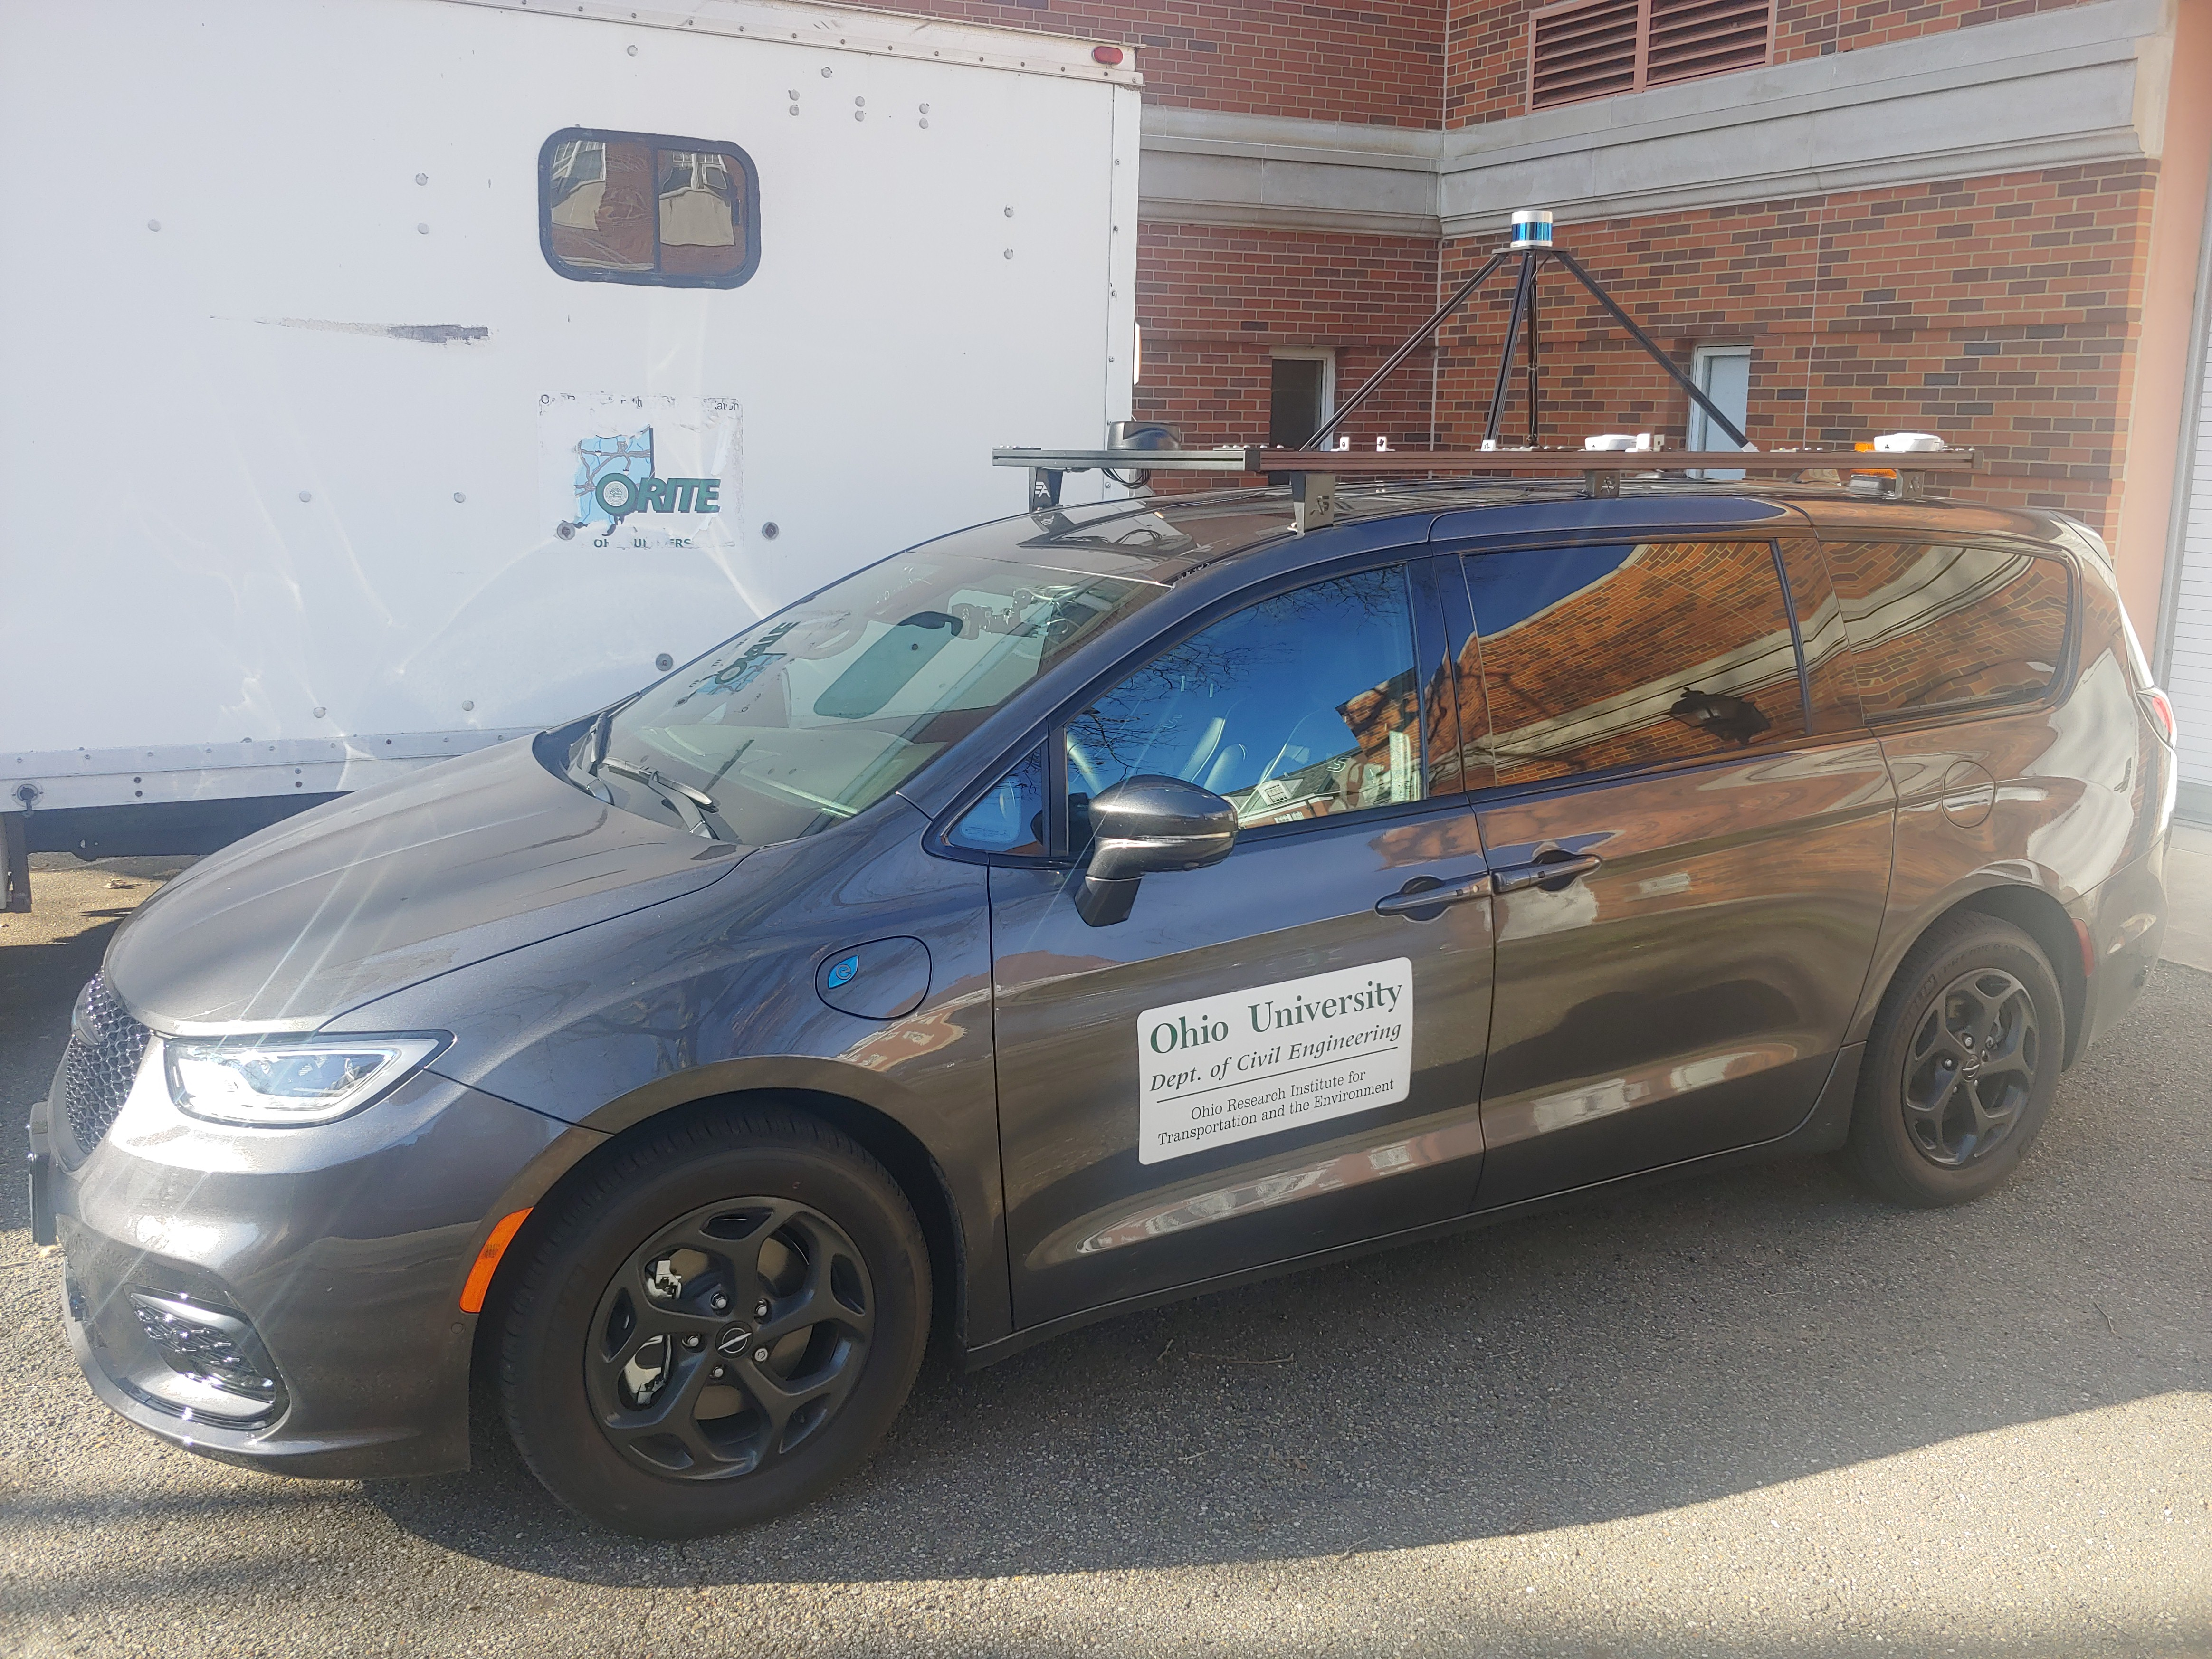
\includegraphics[width=0.9\linewidth,height=4.60 cm,keepaspectratio]{figures/van_on_van}
			\caption[Sensor Van]{}
			\label{fig:van}
		\end{subfigure}
		\begin{subfigure}{0.45\textwidth}
			\centering
			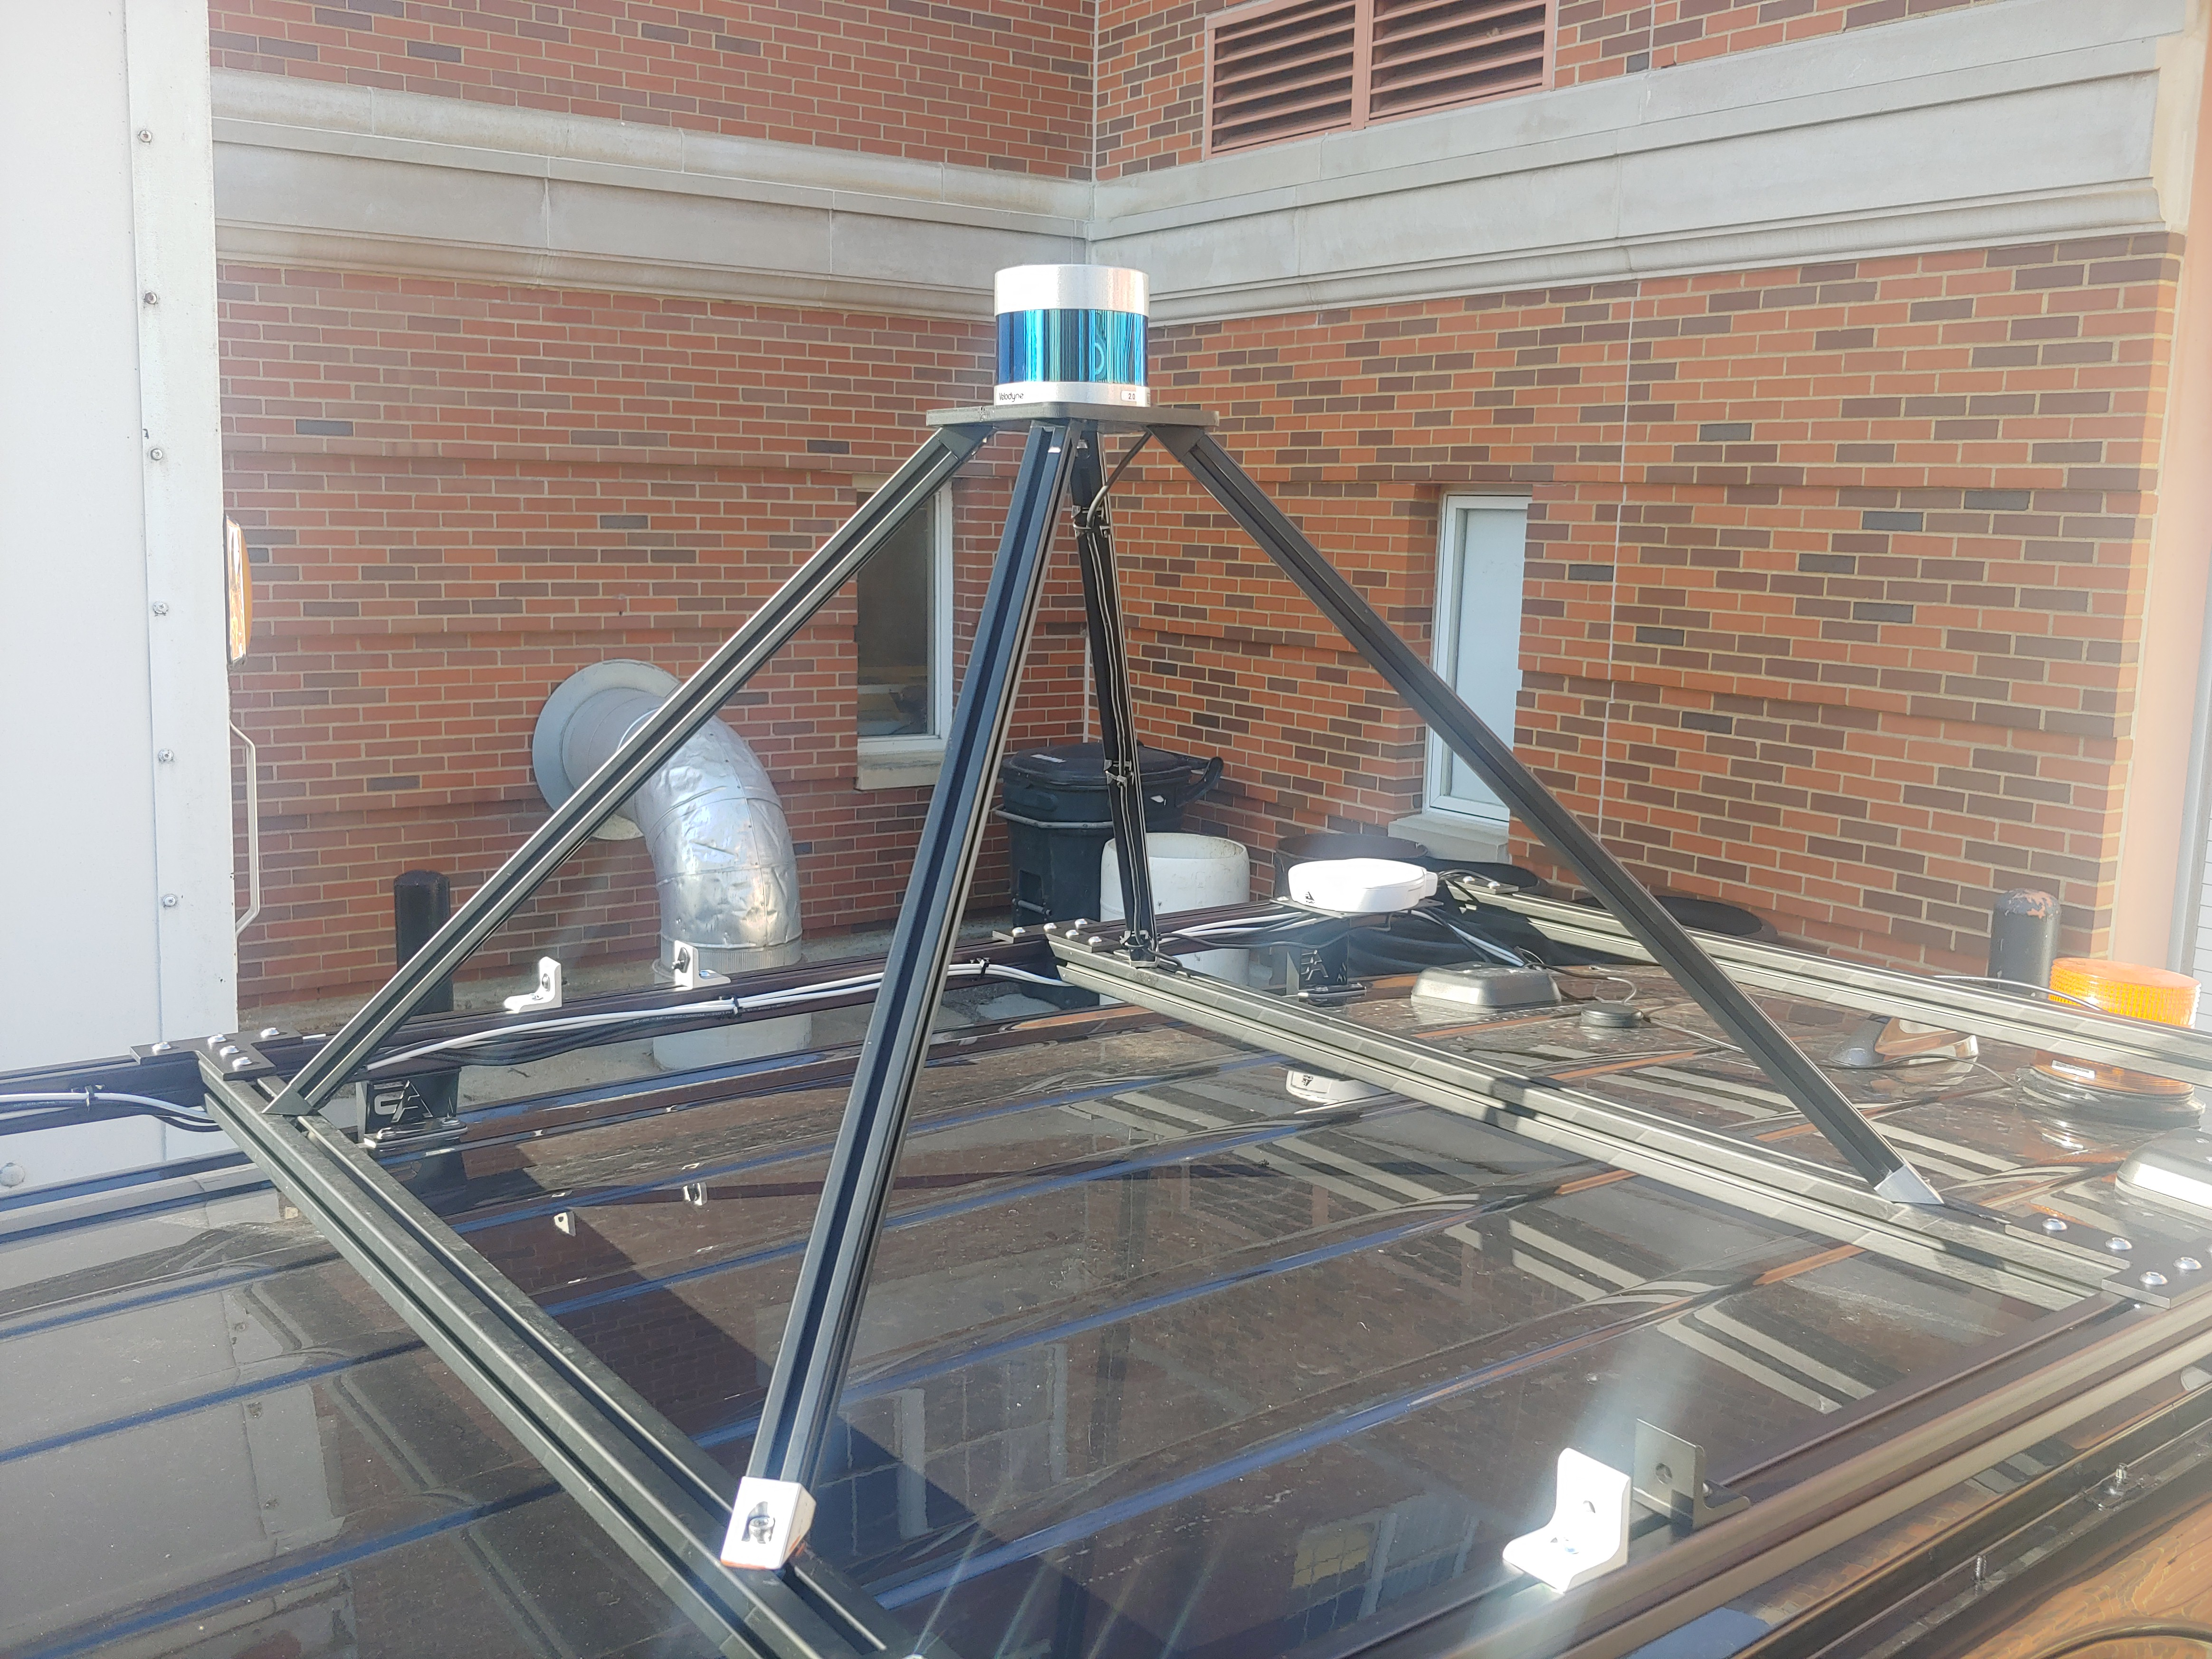
\includegraphics[width=0.9\linewidth,height=4.60 cm,keepaspectratio]{figures/LiDAR_on_van}
			\caption[VLP 32 on Van]{}
			\label{fig:vlp32mount}
		\end{subfigure}
		\caption[Experimental Apparatus]{Experimental Apparatus (a). Velodyne VLP-32 Scanning LiDAR is mounted on top of the vehicle (b).}
		\label{fig:Experimental_Apperatus}
	\end{figure}

	\begin{figure}[H]
		\centering
		\begin{subfigure}{0.45\textwidth}
			\centering
			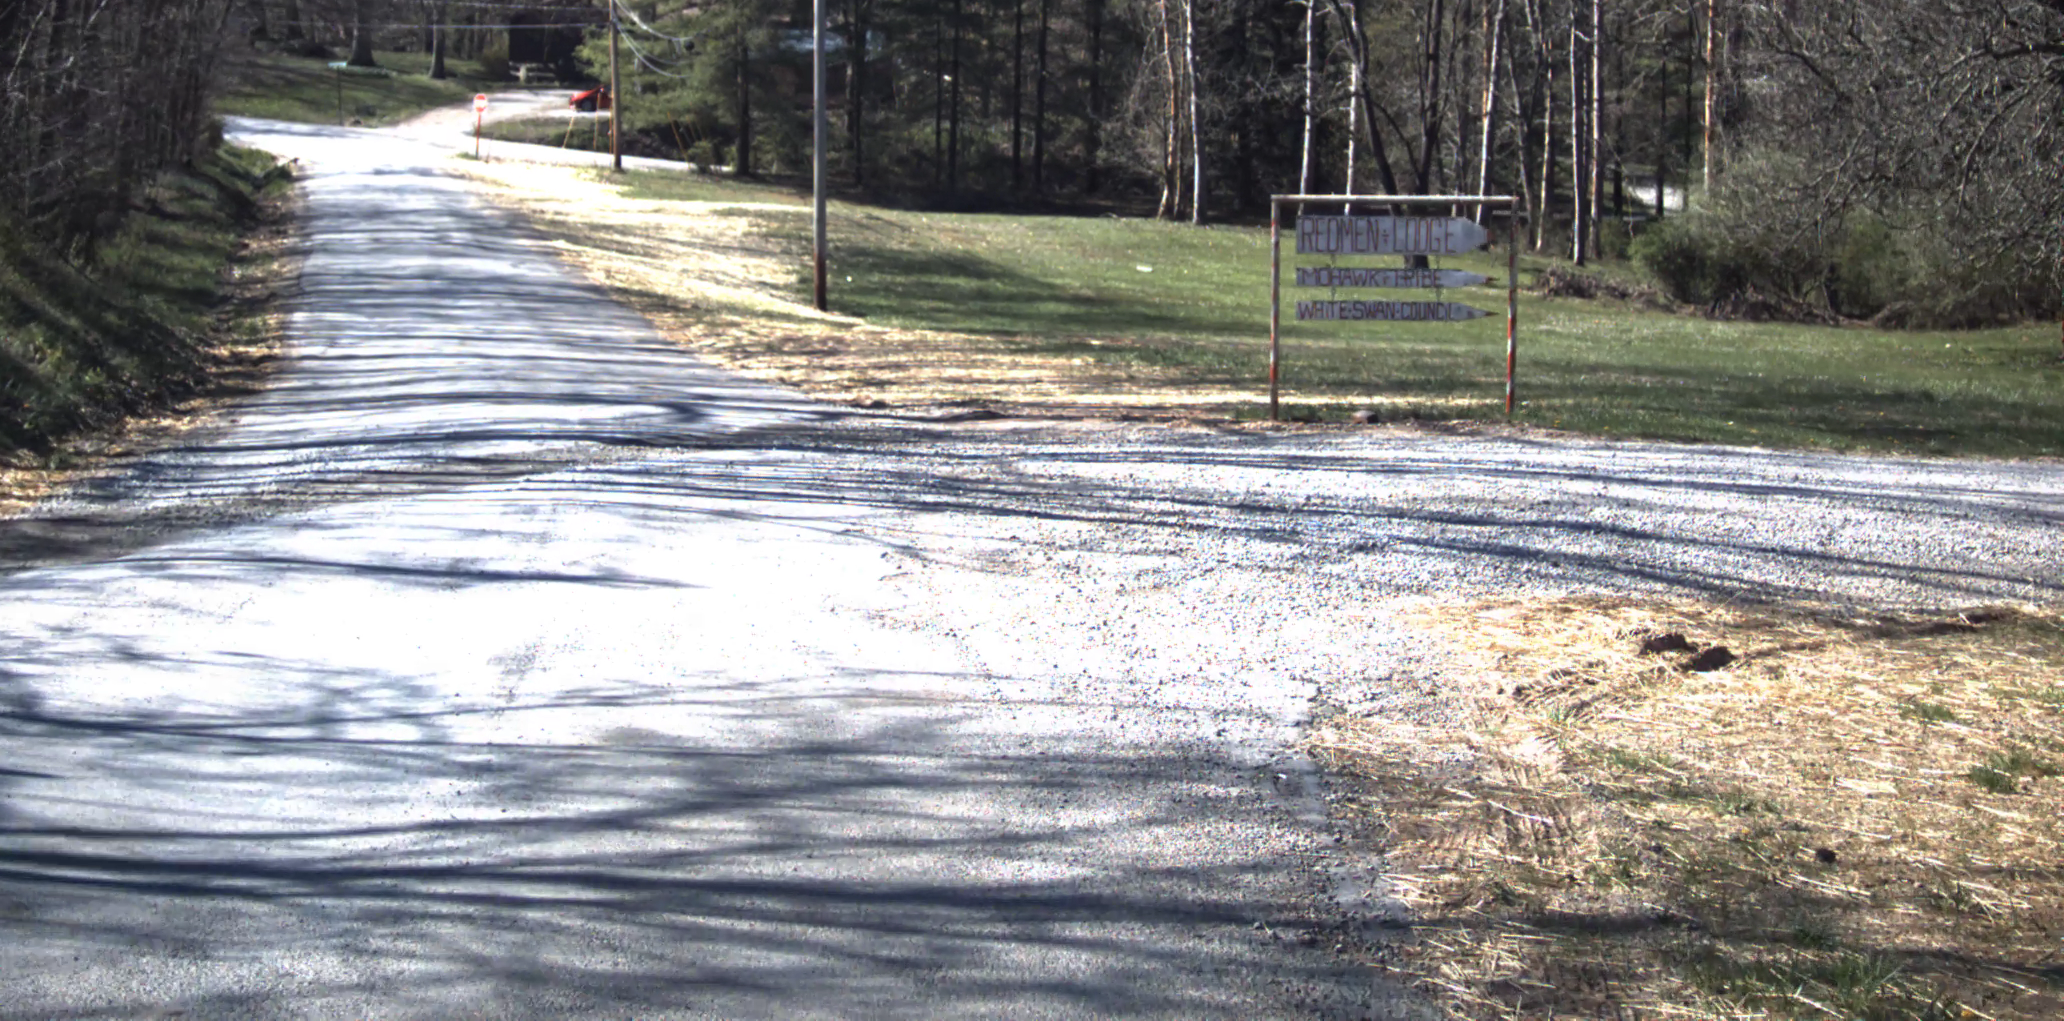
\includegraphics[width=1.0\linewidth,height=5.0 cm,keepaspectratio]{figures/vlcsnap-2023-04-20-08h48m17s447}
			\caption[Blackburn Road Camera View]{}
			\label{fig:Blackburn_Road_View}
		\end{subfigure}
		\begin{subfigure}{0.45\textwidth}
			\centering
			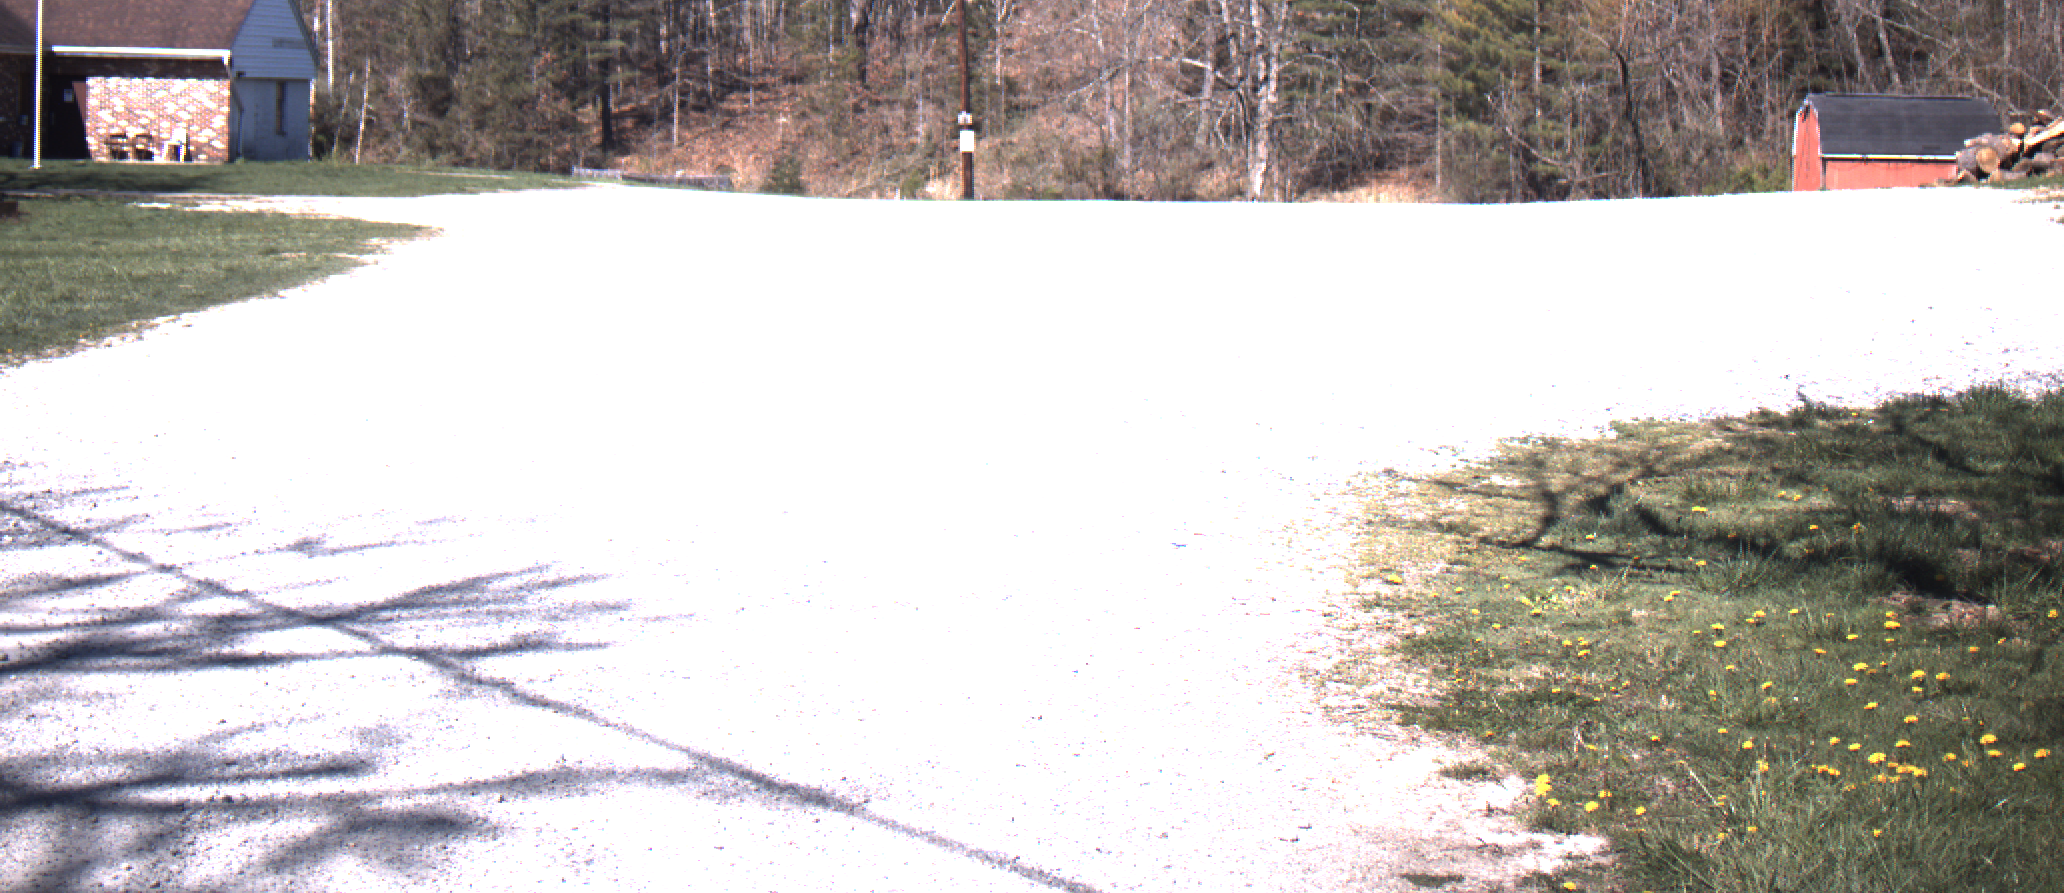
\includegraphics[width=1.0\linewidth,height=5.0 cm,keepaspectratio]{figures/gravel_lot_pic.png}
			\caption[Armig Road Camera View]{}
			\label{fig:Gravel_Lot_View}
		\end{subfigure}
		\caption[Blackburn Road \& Gravel Parking Lot]{Road view of Blackburn Road - an unmarked asphalt road (a). Road view of the gravel driveway (b).}
		\label{fig:Combined_Roads}
	\end{figure}

	{MATLAB was used to process the gathered rosbag files using the their ROSBAG library. Rosbags were directly loaded into the MATLAB environment. Point cloud, GPS, and IMU topics were defined, and the messages were read from the topic and imported. Cartesian coordinates, longitude, latitude, altitude, roll, pitch, and yaw were extracted from the messages.}
	
	{Scanning LiDAR training data was extracted from manually defined gravel, asphalt, and unknown terrain areas on compiled point clouds. Compiling LiDAR data into a single point cloud was completed by post processing rosbags that contained scanning LiDAR, GPS, and IMU data of an unmarked road. Point cloud translation and rotation was accomplished using transformation matrices derived from GPS and IMU data. Rotation matrices were created using extracted roll, pitch, and yaw data from the IMU. LiDAR origin was found using GPS longitude, latitude, and altitude data. Physical distances between the GPS, IMU, and LiDAR was rectitude by obtaining reference frames provided by AutonomouStuff. GPS coordinates were offset by the current orientation and converts the ground truth to the LiDAR frame. GPS, IMU, and LiDAR reference frames and rotational updates were combined into trajectory vectors. Consecutive point cloud scans may then translated and rotated with derived transformation matrices (Figure \ref{fig:Compiled_PCD}). While not as robust as more sophisticated methods of point cloud aggregation such as NDT or ICP scan matching, over shorter distances using this method proved to be adequate for scoring purposes. Manually defined areas may then be overlayed unto the point cloud (Figure \ref{fig:Combined_Classified_PCD}). Six degree arcs from the first three channels of scanning LiDAR data that lay directly in front of the vehicle were extracted and exported to a database if coincident with the manually defined areas.}
	
	\begin{figure}[H]
		\centering
		\begin{subfigure}{0.45\textwidth}
			\centering
			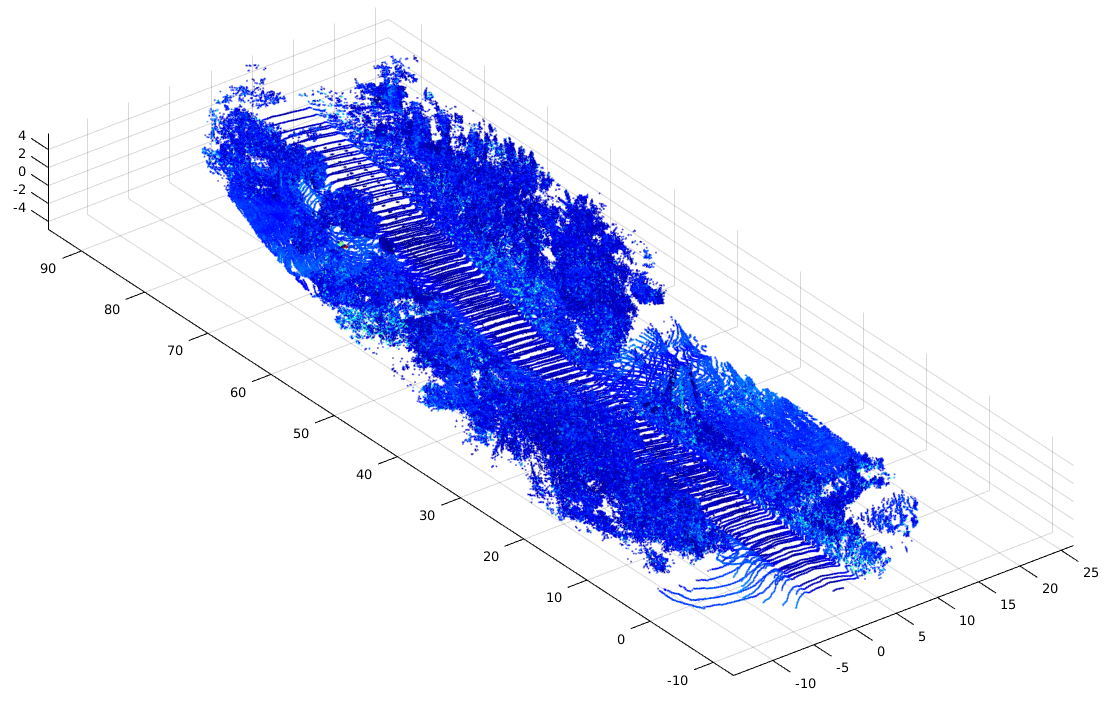
\includegraphics[width=0.95\linewidth]{figures/Compiled_PCD}
			\caption[C]{}
			\label{fig:Compiled_PCD}
		\end{subfigure}
		\begin{subfigure}{0.45\textwidth}
			\centering
			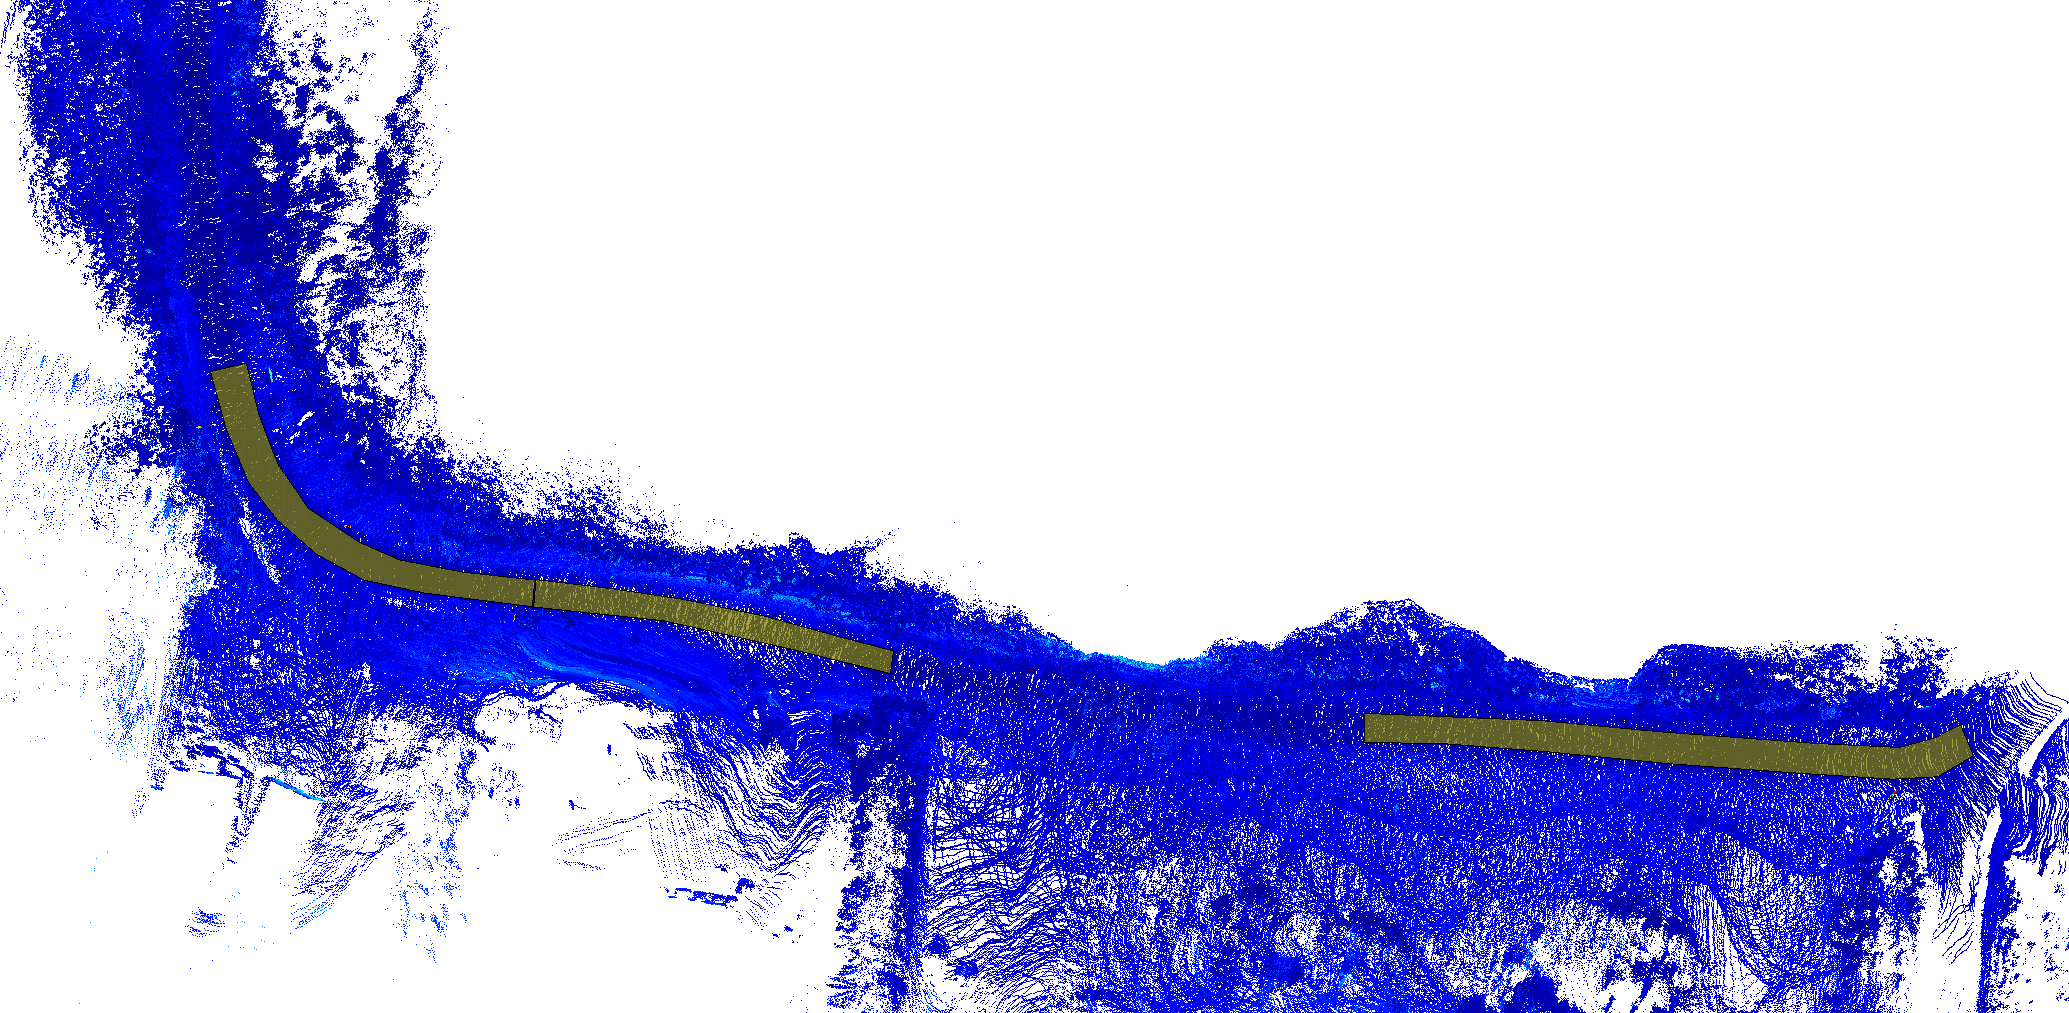
\includegraphics[width=0.95\linewidth]{figures/Manually_Defined_Area_Train_Dat_Grab_2}
			\caption[]{}
			\label{fig:Classified_Areas_PCD}
		\end{subfigure}
		\caption[Compiled and Classified Point Cloud Data]{Point cloud of scanning LiDAR data using GPS and IMU data to determine point of origin and orientation for the LiDAR was used to create a combined point cloud map (a). Manually defined areas inform where training data lies (b).}
		\label{fig:Combined_Classified_PCD}
	\end{figure}
	
%	{RANSAC was implementing by a built-in MATLAB function, $pcfitplane$. Method of Least Squares was implemented by importing a MATLAB library \cite{noauthor_object-oriented_nodate}. Point clouds are individually imported into the MATLAB environment. RANSAC or Method of Least Squares may be used to project a reference plane unto the point cloud. Displaying the point cloud is completed using MATLAB's $pcshow$ function. Training data is selected by manually drawing an area around appropriate points of a desired terrain type using MATLAB's $drawrectangle$ function (Figure \ref{fig:Rectangle_ROI}). Indices for the rectangle are extracted, and MATLAB's function $findPointsInROI$ is used to extract sympatric points within the drawn rectangle. Captured points are then saved to disk along with the projected plane's normal vector and distance from the origin $[a,b,c,d]$.}

%	\begin{figure}[H]
%		\centering
%		\begin{minipage}[c]{.45\linewidth}
%			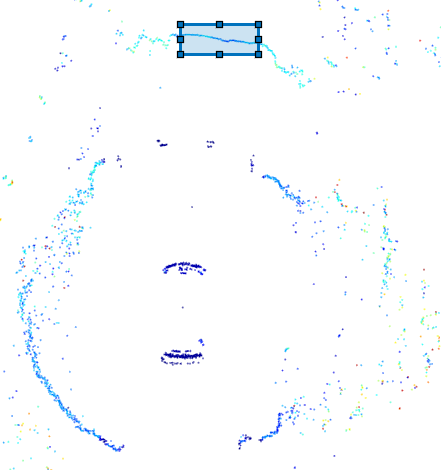
\includegraphics[width=.95\linewidth]{figures/Rectangle_ROI}
%			\caption[Region of Interest Selection]{MATLAB was used to select training data using the $drawrectangle$ function and extracting points that lay within the defined area.}
%			\label{fig:Rectangle_ROI}
%		\end{minipage}
%		\hfill
%		\begin{minipage}[c]{0.45\linewidth}
%			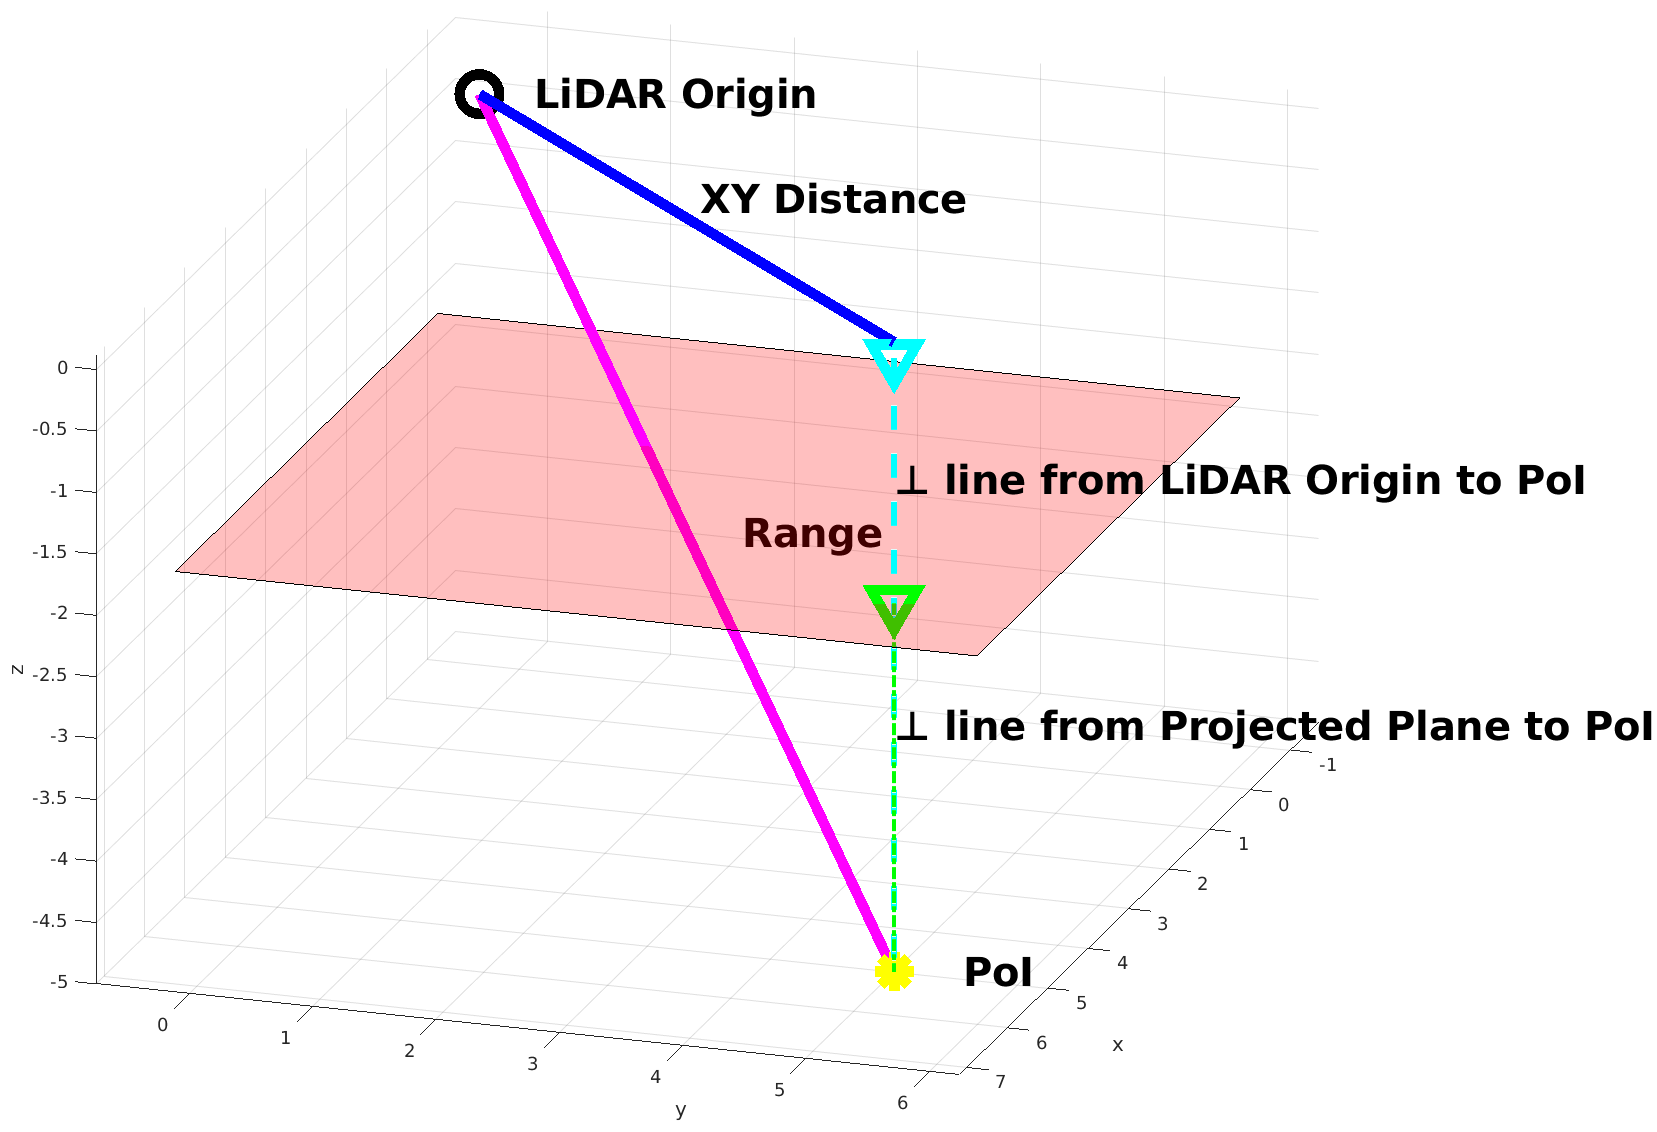
\includegraphics[width=.95\linewidth]{figures/xy_vs_range}
%			\caption[XY vs Range vs Z Height]{Three references for feature extraction may be seen in this simplified graph. First is the Range shown by the magenta line from the LiDAR origin to the Point of Interest (PoI). Second is the height from  LiDAR origin to the PoI (cyan). Finally, distance from the projected plane (red) to the PoI (green). XY Distance (blue) and Range (magenta) from the sensor was used consider the effect of distance from LiDAR origin to the PoI.}
%			\label{fig:xy_vs_range}
%		\end{minipage}
%	\end{figure}


	{Feature extraction was completed by performing mathematical functions on the gathered spatial and remission training data. Standard Deviation ($\sigma$), Roughness ($max - min$), Min-Max Ratio ($min / max$), Min$^{2}$-Max Ratio ($min^2 / max$), and Gradient ($sqrt(\sum_{1}^{n} G))$), where $G$ is an $1*n$ array comprising of the differences between consecutive points in the spatial or remission data array. Features were non-dimensionalized as necessary by dividing by the average range of the arc to LiDAR point of origin to the appropriate power. Thirty percent of the training data was randomly selected and reserved to create a validation data set.} 
	
	{MATLAB's Classification Learner Application was used to generate a Random Decision Forests for each considered scanning LiDAR channel. Decision tree depth, number of learners, and number of features to consider for each binary split are hyper-parameters that were optimized using MATLAB's Bayesian Optimization.}

	{Classifying consecutive LiDAR scans was accomplished by examination of nine arcs of interest in front and forty-five degree angles left and right from the front of the experimental apparatus. Features from each arc were extracted and the arc was classified. Averaged x, y, and z coordinates were taken of each arc and projected unto a manually defined truth area map (Figure \ref{fig:Classified_Areas_PCD}). Accuracy scores of each area was calculated, allowing evaluation of road detection performance.}
	
	
\section{Results}
	
	{Five drive-bys of Blackburn Road with three intercepting gravel parking lots and driveways were completed and scanning LiDAR, GPS, and IMU data was collected. Training data was generated using MATLAB to extract LiDAR data from rosbags. Random Decision Forests classification algorithms were generated. Testing consecutive scans was completed by post processing rosbags that contained scanning LiDAR, GPS, and IMU data. Physical distances between the GPS, IMU, and LiDAR were rectified by measuring the distance between the modules. Rotational reference frames between the GPS, IMU, and LiDAR were rectified by applying appropriate rotational matrices. Transformation matrices were created by considering the GPS position and the IMU's roll, pitch, and yaw data. Three scanning LiDAR arcs from three channels in front of the vehicle were classified. Translation and rotation was applied to the averaged x, y, and z coordinates of each arc's terrain classification results. Consecutive scanning LiDAR data was projected on manually classified truth areas representing road road surfaces (Figure \ref{fig:area_percentages}) and percentages of terrain types per area were calculated. }
		
	{Overall it was found that an average true-positive accuracy of all intercepting gravel surfaces was 67.54\%. If any asphalt miss-classification on the gravel areas is included, the average true-positive road detection accuracy increases to 76.97\%. It was found that an average true-positive accuracy of all asphalt surfaces was 87.05\%. Differentiation between gravel road surfaces and surrounding terrain is necessary to determine boundaries for trajectory tracking and navigation. Side-of-road areas were established (Figure \ref{fig:prepostadjust}), and the overall average for "unknown" terrain type was found to be 77.49\%.}

	\begin{figure}[H]
		\centering
		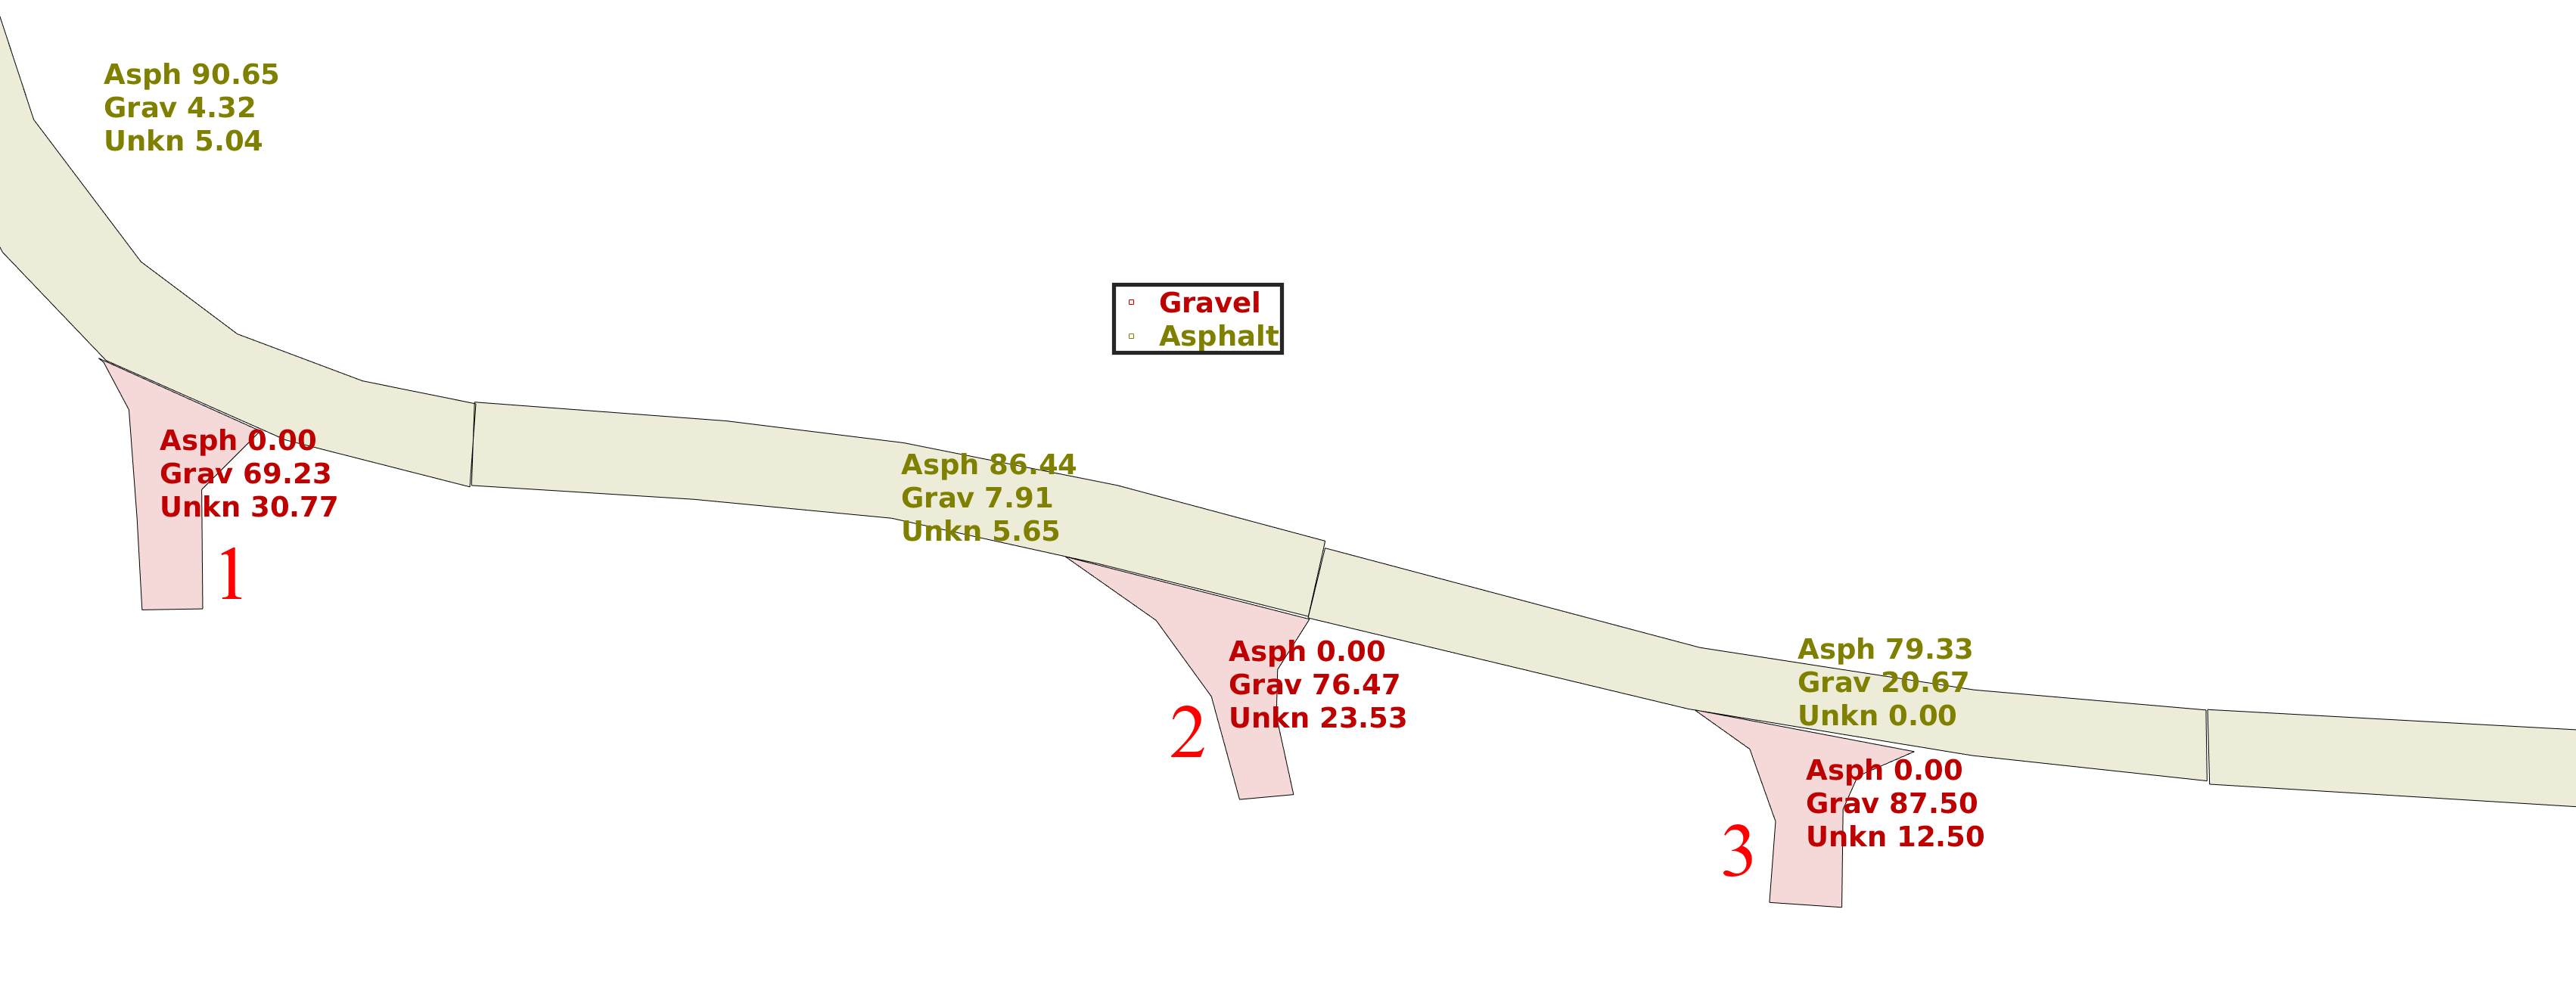
\includegraphics[width=0.9\linewidth]{figures/rm_db_4_percentages_big_anotated}
		\caption[Area Percentage Scores]{Five runs of Blackburn Road with the intercepting gravel parking lot were classified. Shown is the results of one run. Percentages of each terrain type per area were calculated. Area $3$ is the gravel parking lot entrance from which training data was extracted.}
		\label{fig:area_percentages}
	\end{figure}

%	\begin{figure}[H]
%		\centering
%		\begin{subfigure}{0.495\textwidth}
%			\centering
%			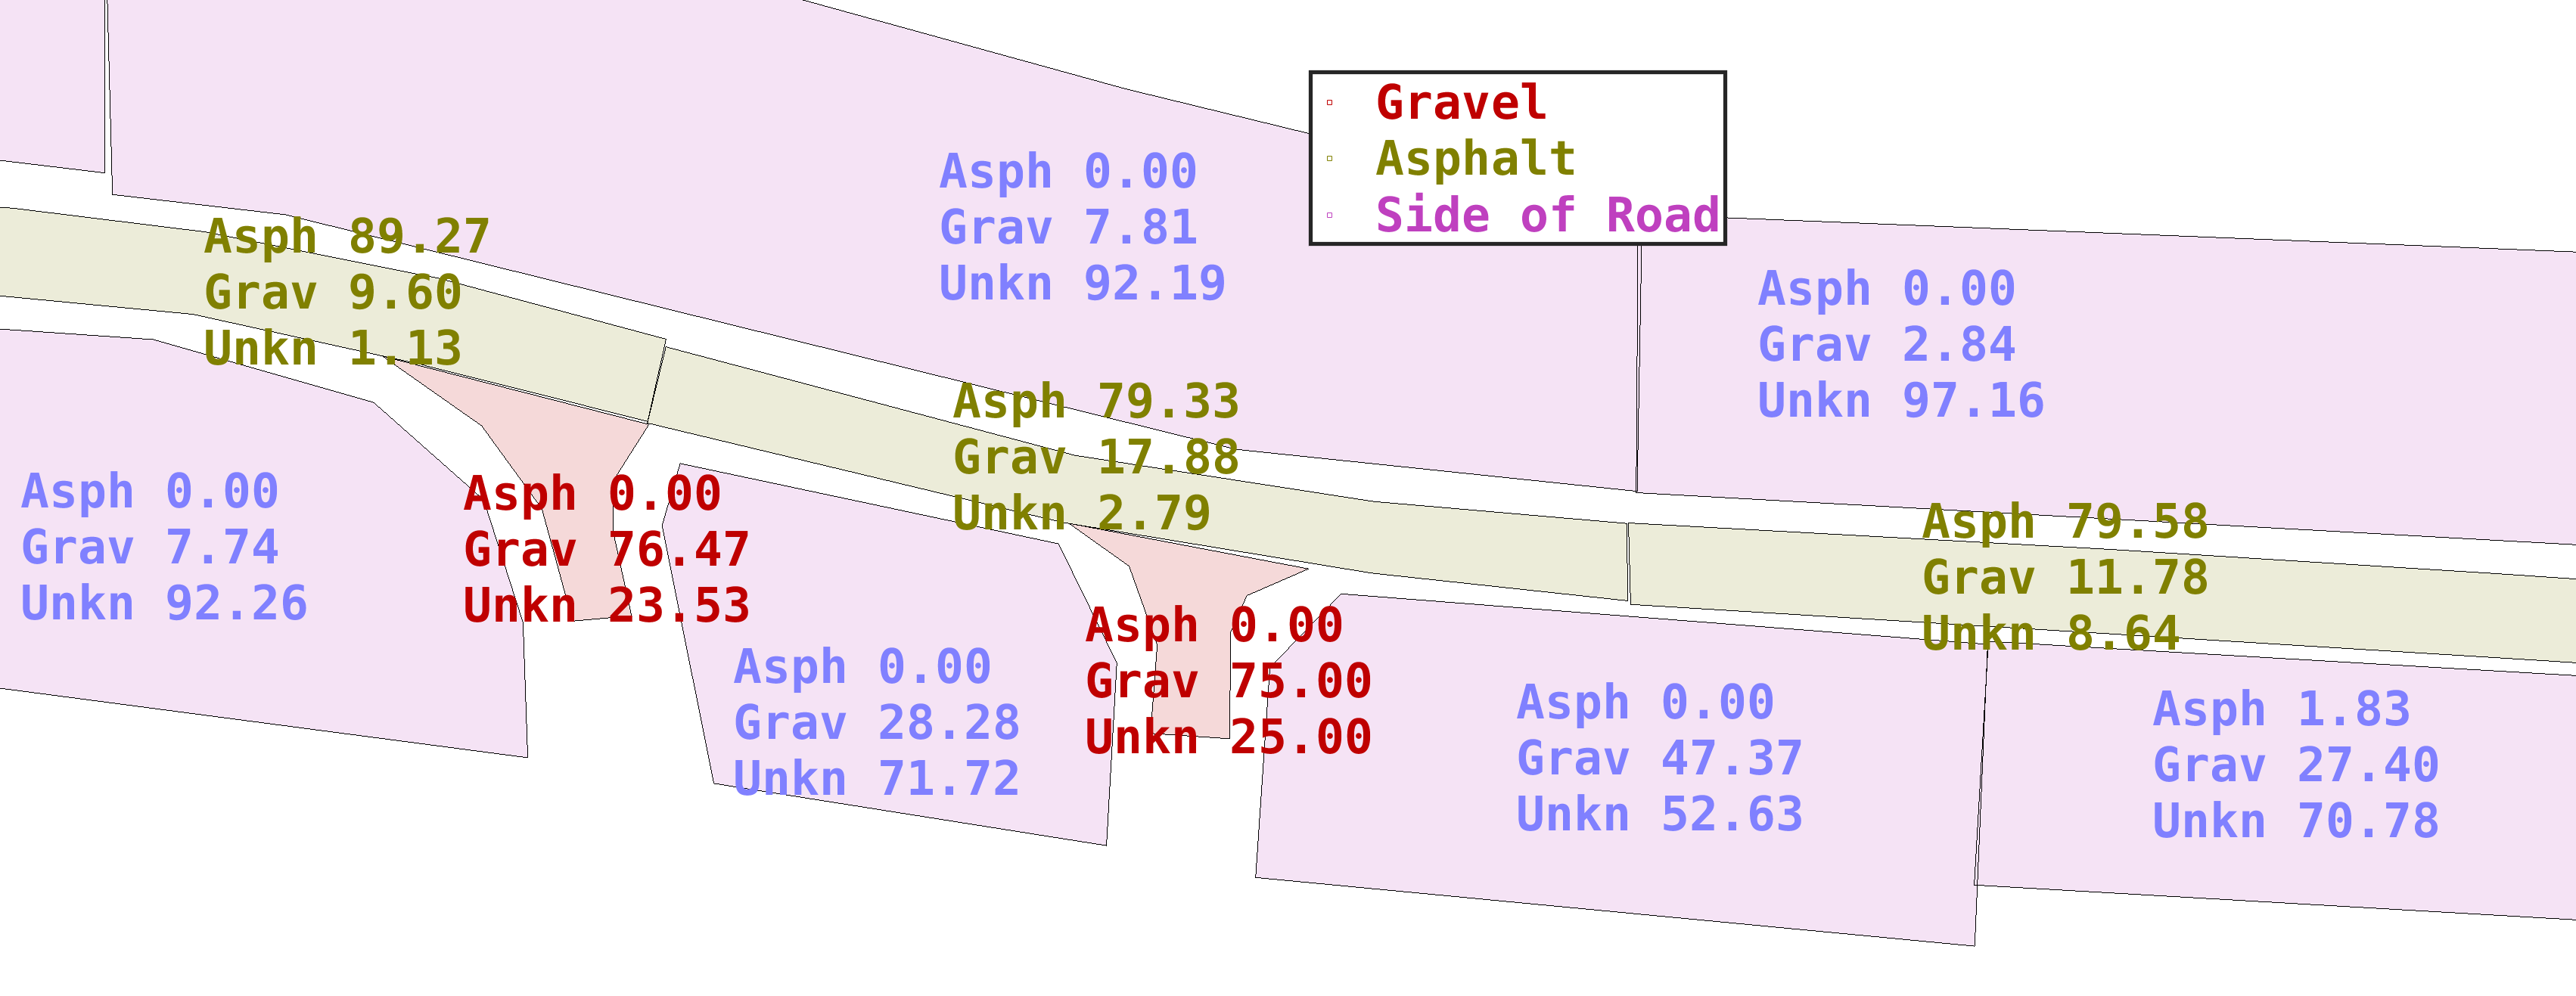
\includegraphics[width=0.975\linewidth]{figures/side_of_road_nums_4_with_no_filts_2}
%			\caption[Pre-Adjusted]{}
%			\label{fig:pre-adjust}	
%		\end{subfigure}
%		\begin{subfigure}{0.495\textwidth}
%			\centering
%			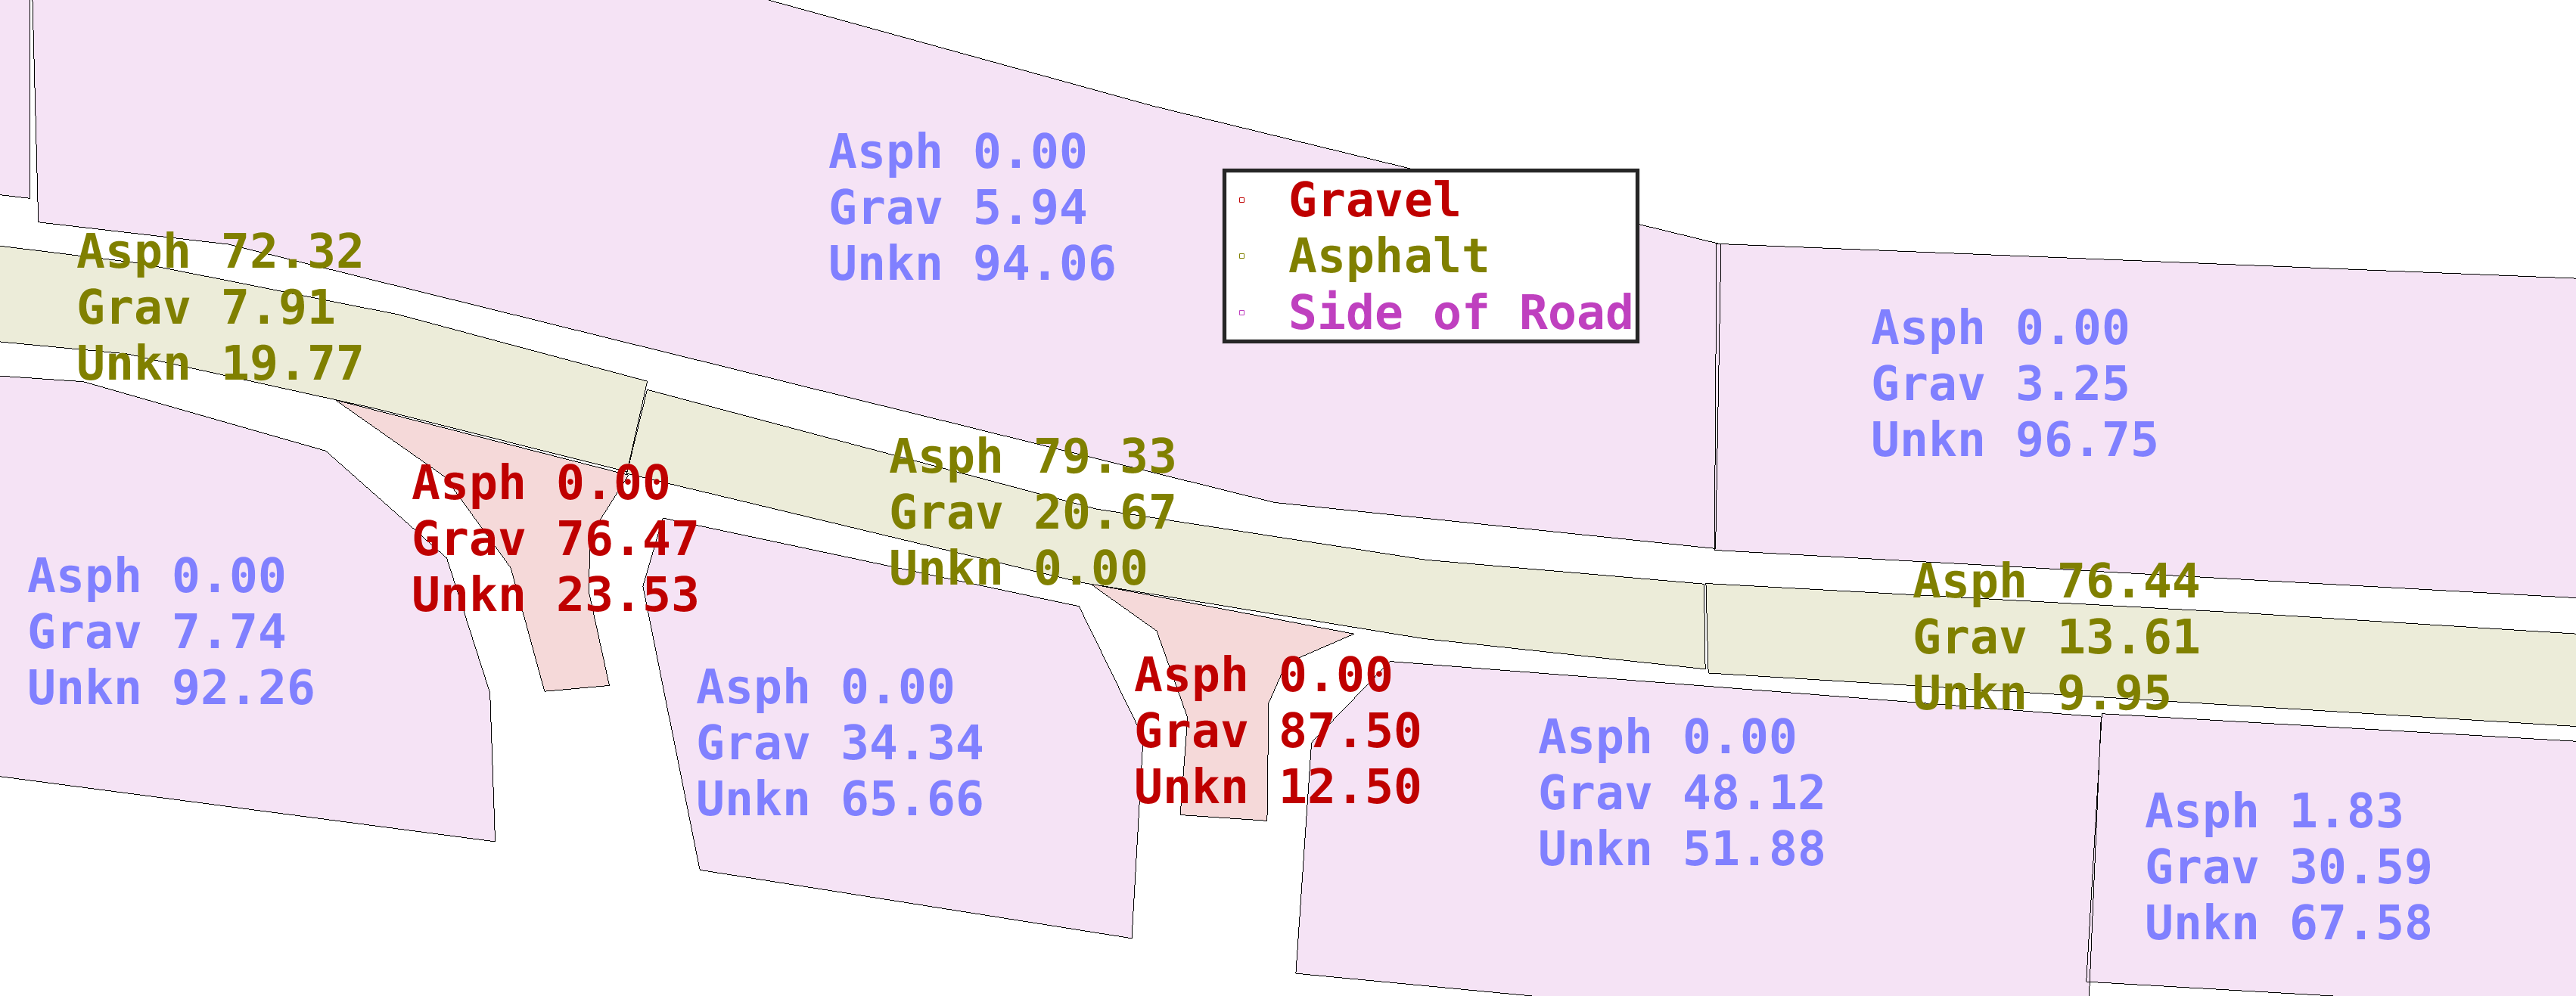
\includegraphics[width=0.975\linewidth]{figures/side_of_road_nums_4_with_filts_2}
%			\caption[Post-Adjusted]{}
%			\label{fig:post-adjust}
%		\end{subfigure}
%		\label{fig:prepostadjust}
%		\caption[Post-Adjusted]{Raw classification result example (a). Results were slightly altered by considering confidence scores and inter-arc distances to decrease miss-classification of gravel surfaces, however the effect was negligible (b).}
%	\end{figure}

	\begin{figure}[H]
			\centering
			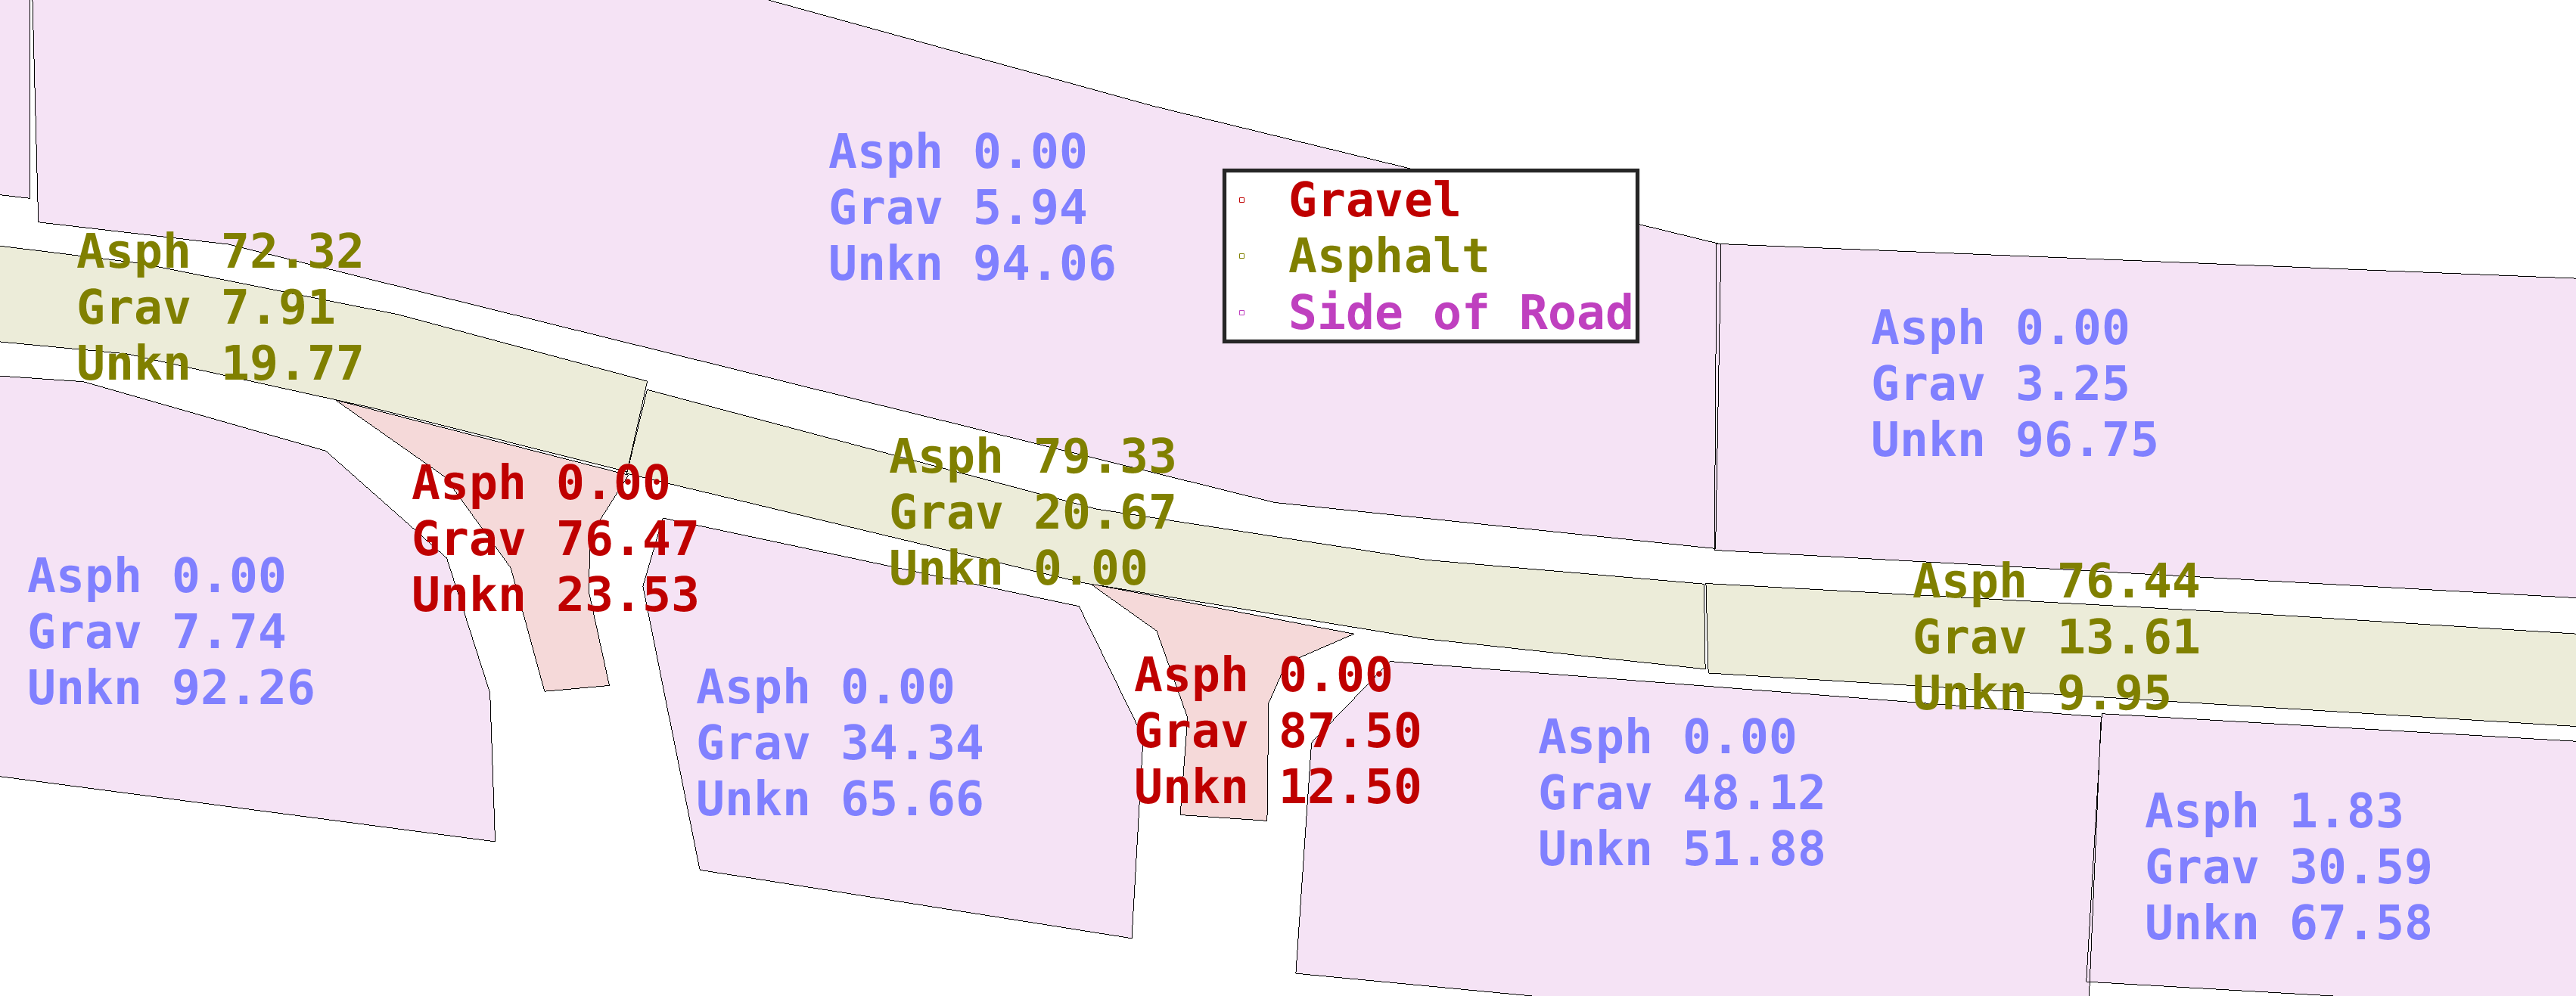
\includegraphics[width=0.975\linewidth]{figures/side_of_road_nums_4_with_filts_2}
			\caption[Post-Adjusted]{}
			\label{fig:prepostadjust}
		\caption[Area Scores]{Per-area scores were calculated, indicating algorithm efficiency of unmarked road detection. }
	\end{figure}

	{Classified point clouds were manually examined for 'best guess' locations for gravel and asphalt surfaces. Two out of three positive gravel identifications must be made on each channel, be evenly spaced, and be relatively co-planar to other road surface guesses in order for a positive guess for an asphalt or gravel surface to be made (Figure \ref{fig:rm_db_4_toc}). Driveways $1$ and $2$ were detected in all five drive-bys, driveway $3$ was detected in four leading to an 91.67\% accuracy in intercepting gravel road detection. It was found that in three drive-bys there was a false positive driveway detection, however the location of the false-positive was not repeated. In all drive-bys the asphalt road was accurately detected. }
	
	{Classification was completed using Ubuntu 18.04 and an AMD Ryzen 9 5900X 12 core 24 thread. Rate of classification for all nine areas of interest in a single scan was found to be an average of 1.226 seconds using a single core. Further optimization may increase this speed, however real-time classification is not a focus of this work. Using all cores when processing a ROSBAG file indicated that a rate of 55.81 feet per second or 38.05 miles per hour was accomplished.}
	
	\begin{figure}[H]
		\centering
		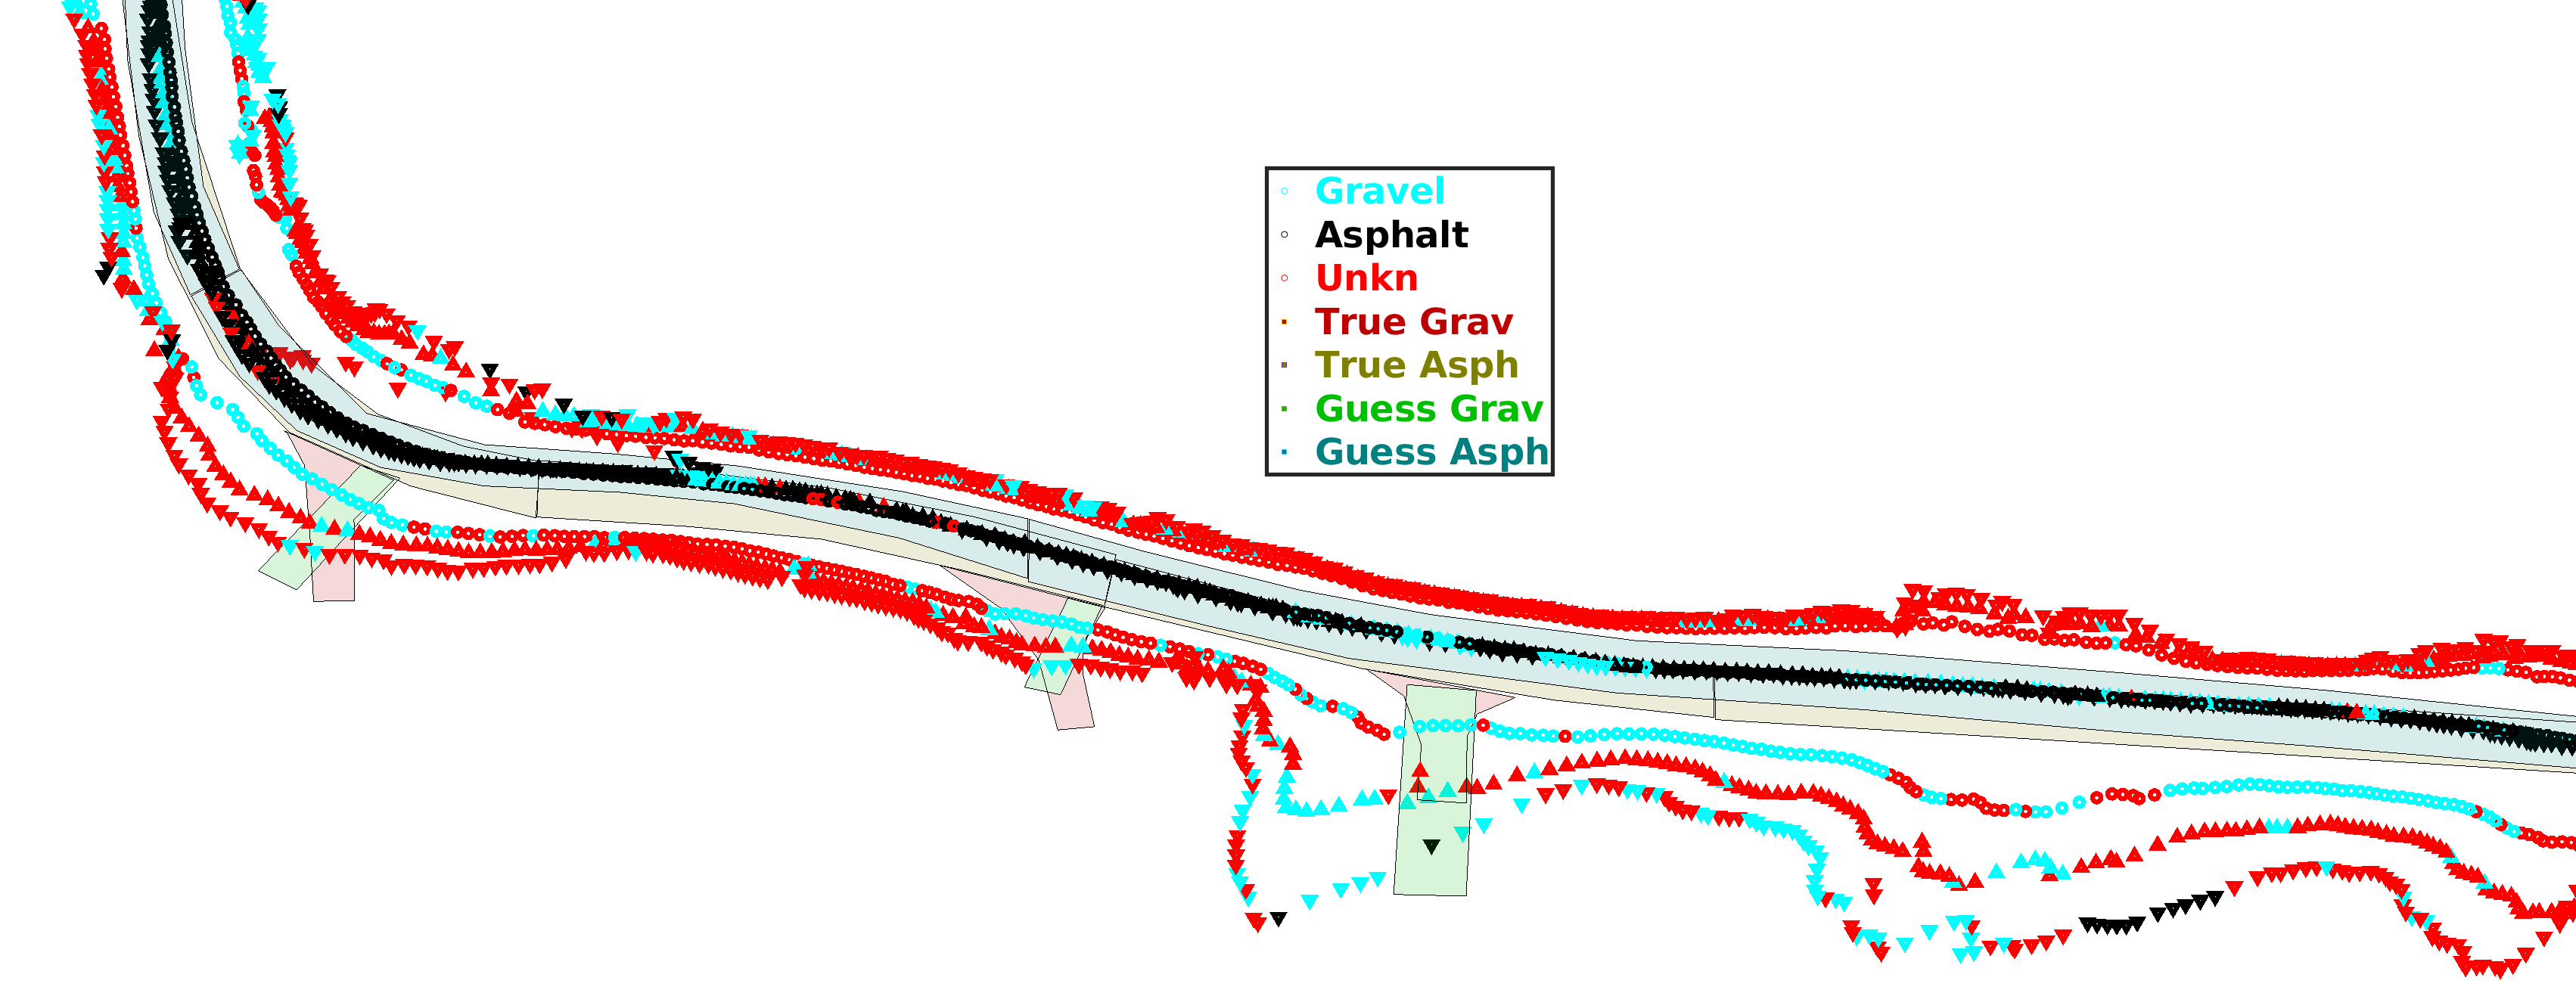
\includegraphics[width=0.9\linewidth]{figures/rm_db_4_toc}
		\caption[Projected Guess vs Truth]{Gravel and asphalt surfaces were manually guessed using a rule set and compared to actual road-surface areas. }
		\label{fig:rm_db_4_toc}
	\end{figure}

\section{Discussion}

	
	{Classification of real-world data outside of the training data set presents difficulties to the generated Random Decision Forest Classifiers generated in this work. Due to the side of the road was being re-grassed near area $3$ (Figure \ref{fig:area_percentages}, Figure \ref{fig:Blackburn_Road_View}), the algorithm struggled to differentiate the dirt from gravel, leading to some miss-classification of the side-of-road areas. Examination of the feature distribution shows a high amount of overlap (Figure \ref{}). Exploitation of confidence scores to adjust results by requiring a very high confidence for positive gravel surface classification was explored. All gravel surfaces that did not meet a 80\% confidence score was re-labeled as "unknown", however these adjustment had either a negligible or detrimental impact on the final results. Higher confidence score requirements resulted in "unknown" over-classification, while too low resulted in "gravel" over-classification.  }
	
	
	
	
\section{Conclusion}
	
	% Summary of Work & Closing Statements
	{High definition scanning LiDAR and GPS data was gathered on Blackburn Road and an intercepting gravel lot in Athens Ohio. Properties describing surface roughness and remission data were extracted and used to train Random Decision Forests. Terrain classification of consecutive scans compared to manually defined road surface areas yielded accuracy scores for gauging algorithm capability for gravel surface detection. It was found that a true-positive accuracy for gravel and asphalt surfaces was 67.54\% and 87.05\% respectively. Classified point clouds were manually examined and gravel areas were projected and compared with actual gravel surface areas. Overlapping results between manually projected and actual road surface areas resulted in 91.67\% intercepting gravel road detection accuracy. In conjunction with the overlapping areas and the high true-positive detection accuracy of gravel surfaces, this method of gravel road detection is a promising method of gravel road surface detection. This work addressed the problem of road surface detection on unmarked gravel and chipseal roads. Current LiDAR and Camera based detection models were insufficient due to lack of distinct features typical of urban roads, such as painted line markings or curbs, or have excessive computational or storage requirements. This work balanced accuracy and efficiency by using less intensive analysis techniques of smaller point cloud data sets. The described work was a method of detecting physical unmarked gravel and chipseal roads by using a terrain classification approach to predicting road surface area. The impact of this work is that autonomous vehicles using LiDAR may be able to detect unmarked gravel and chipseal road surfaces, allowing autonomous operations on 1.5 million miles of previously undetected rural roads.} 
	
	
% For peer review papers, you can put extra information on the cover
% page as needed:
% \ifCLASSOPTIONpeerreview
% \begin{center} \bfseries EDICS Category: 3-BBND \end{center}
% \fi
%
% For peerreview papers, this IEEEtran command inserts a page break and
% creates the second title. It will be ignored for other modes.
\IEEEpeerreviewmaketitle




% if have a single appendix:
%\appendix[Proof of the Zonklar Equations]
% or
%\appendix  % for no appendix heading
% do not use \section anymore after \appendix, only \section*
% is possibly needed

% use appendices with more than one appendix
% then use \section to start each appendix
% you must declare a \section before using any
% \subsection or using \label (\appendices by itself
% starts a section numbered zero.)
%


\appendices
%\section{Equations}

%\begin{equation}\label{eqn:MLS}
%	\left[ {\begin{array}{cc}
%			\sum_{i=1}^{m} x_i z_i \\
%			\sum_{i=1}^{m} y_i z_i \\
%			\sum_{i=1}^{m} z_i \\
%			
%	\end{array} } \right]
%	=
%	\left[ {\begin{array}{ccc}
%			\sum_{i=1}^{m} x_i^2 		& \sum_{i=1}^{m} x_i y_i 		& \sum_{i=1}^{m} x_i \\
%			\sum_{i=1}^{m} x_i y_i 		& \sum_{i=1}^{m} y_i^2 			& \sum_{i=1}^{m} y_i \\
%			\sum_{i=1}^{m} x_i 			& \sum_{i=1}^{m} y_i 			& \sum_{i=1}^{m} 1   \\
%	\end{array} } \right]
%	\left[ {\begin{array}{cc}
%			A\\
%			B\\
%			C\\
%	\end{array} } \right]
%\end{equation}
%\centering
%{Method of Least Squares Planar Projection}


% you can choose not to have a title for an appendix
%% if you want by leaving the argument blank
%\section{}
%Appendix two text goes here.


% use section* for acknowledgment
\justifying
\section*{Acknowledgment}


	{Special thanks to Dr. Jay Wilhelm for his guidance and Travis Moleski for his help in LiDAR map building.}


% Can use something like this to put references on a page
% by themselves when using endfloat and the captionsoff option.
\ifCLASSOPTIONcaptionsoff
\newpage
\fi



% trigger a \newpage just before the given reference
% number - used to balance the columns on the last page
% adjust value as needed - may need to be readjusted if
% the document is modified later
%\IEEEtriggeratref{8}
% The "triggered" command can be changed if desired:
%\IEEEtriggercmd{\enlargethispage{-5in}}

% references section

% can use a bibliography generated by BibTeX as a .bbl file
% BibTeX documentation can be easily obtained at:
% http://mirror.ctan.org/biblio/bibtex/contrib/doc/
% The IEEEtran BibTeX style support page is at:
% http://www.michaelshell.org/tex/ieeetran/bibtex/
%\bibliographystyle{IEEEtran}
% argument is your BibTeX string definitions and bibliography database(s)
%\bibliography{IEEEabrv,../bib/paper}
%
% <OR> manually copy in the resultant .bbl file
% set second argument of \begin to the number of references
% (used to reserve space for the reference number labels box)


	\bibliographystyle{ieeetr}  
	\bibliography{resources.bib} 





% that's all folks
\end{document}